\clearpage
\newpage % 开始新的一页
    \thispagestyle{empty} % 移除本页的页眉和页脚[8,9](@ref)
    \newgeometry{margin=0pt} % 临时将本页的页边距全部设置为0[1](@ref)
    \noindent % 防止缩进
    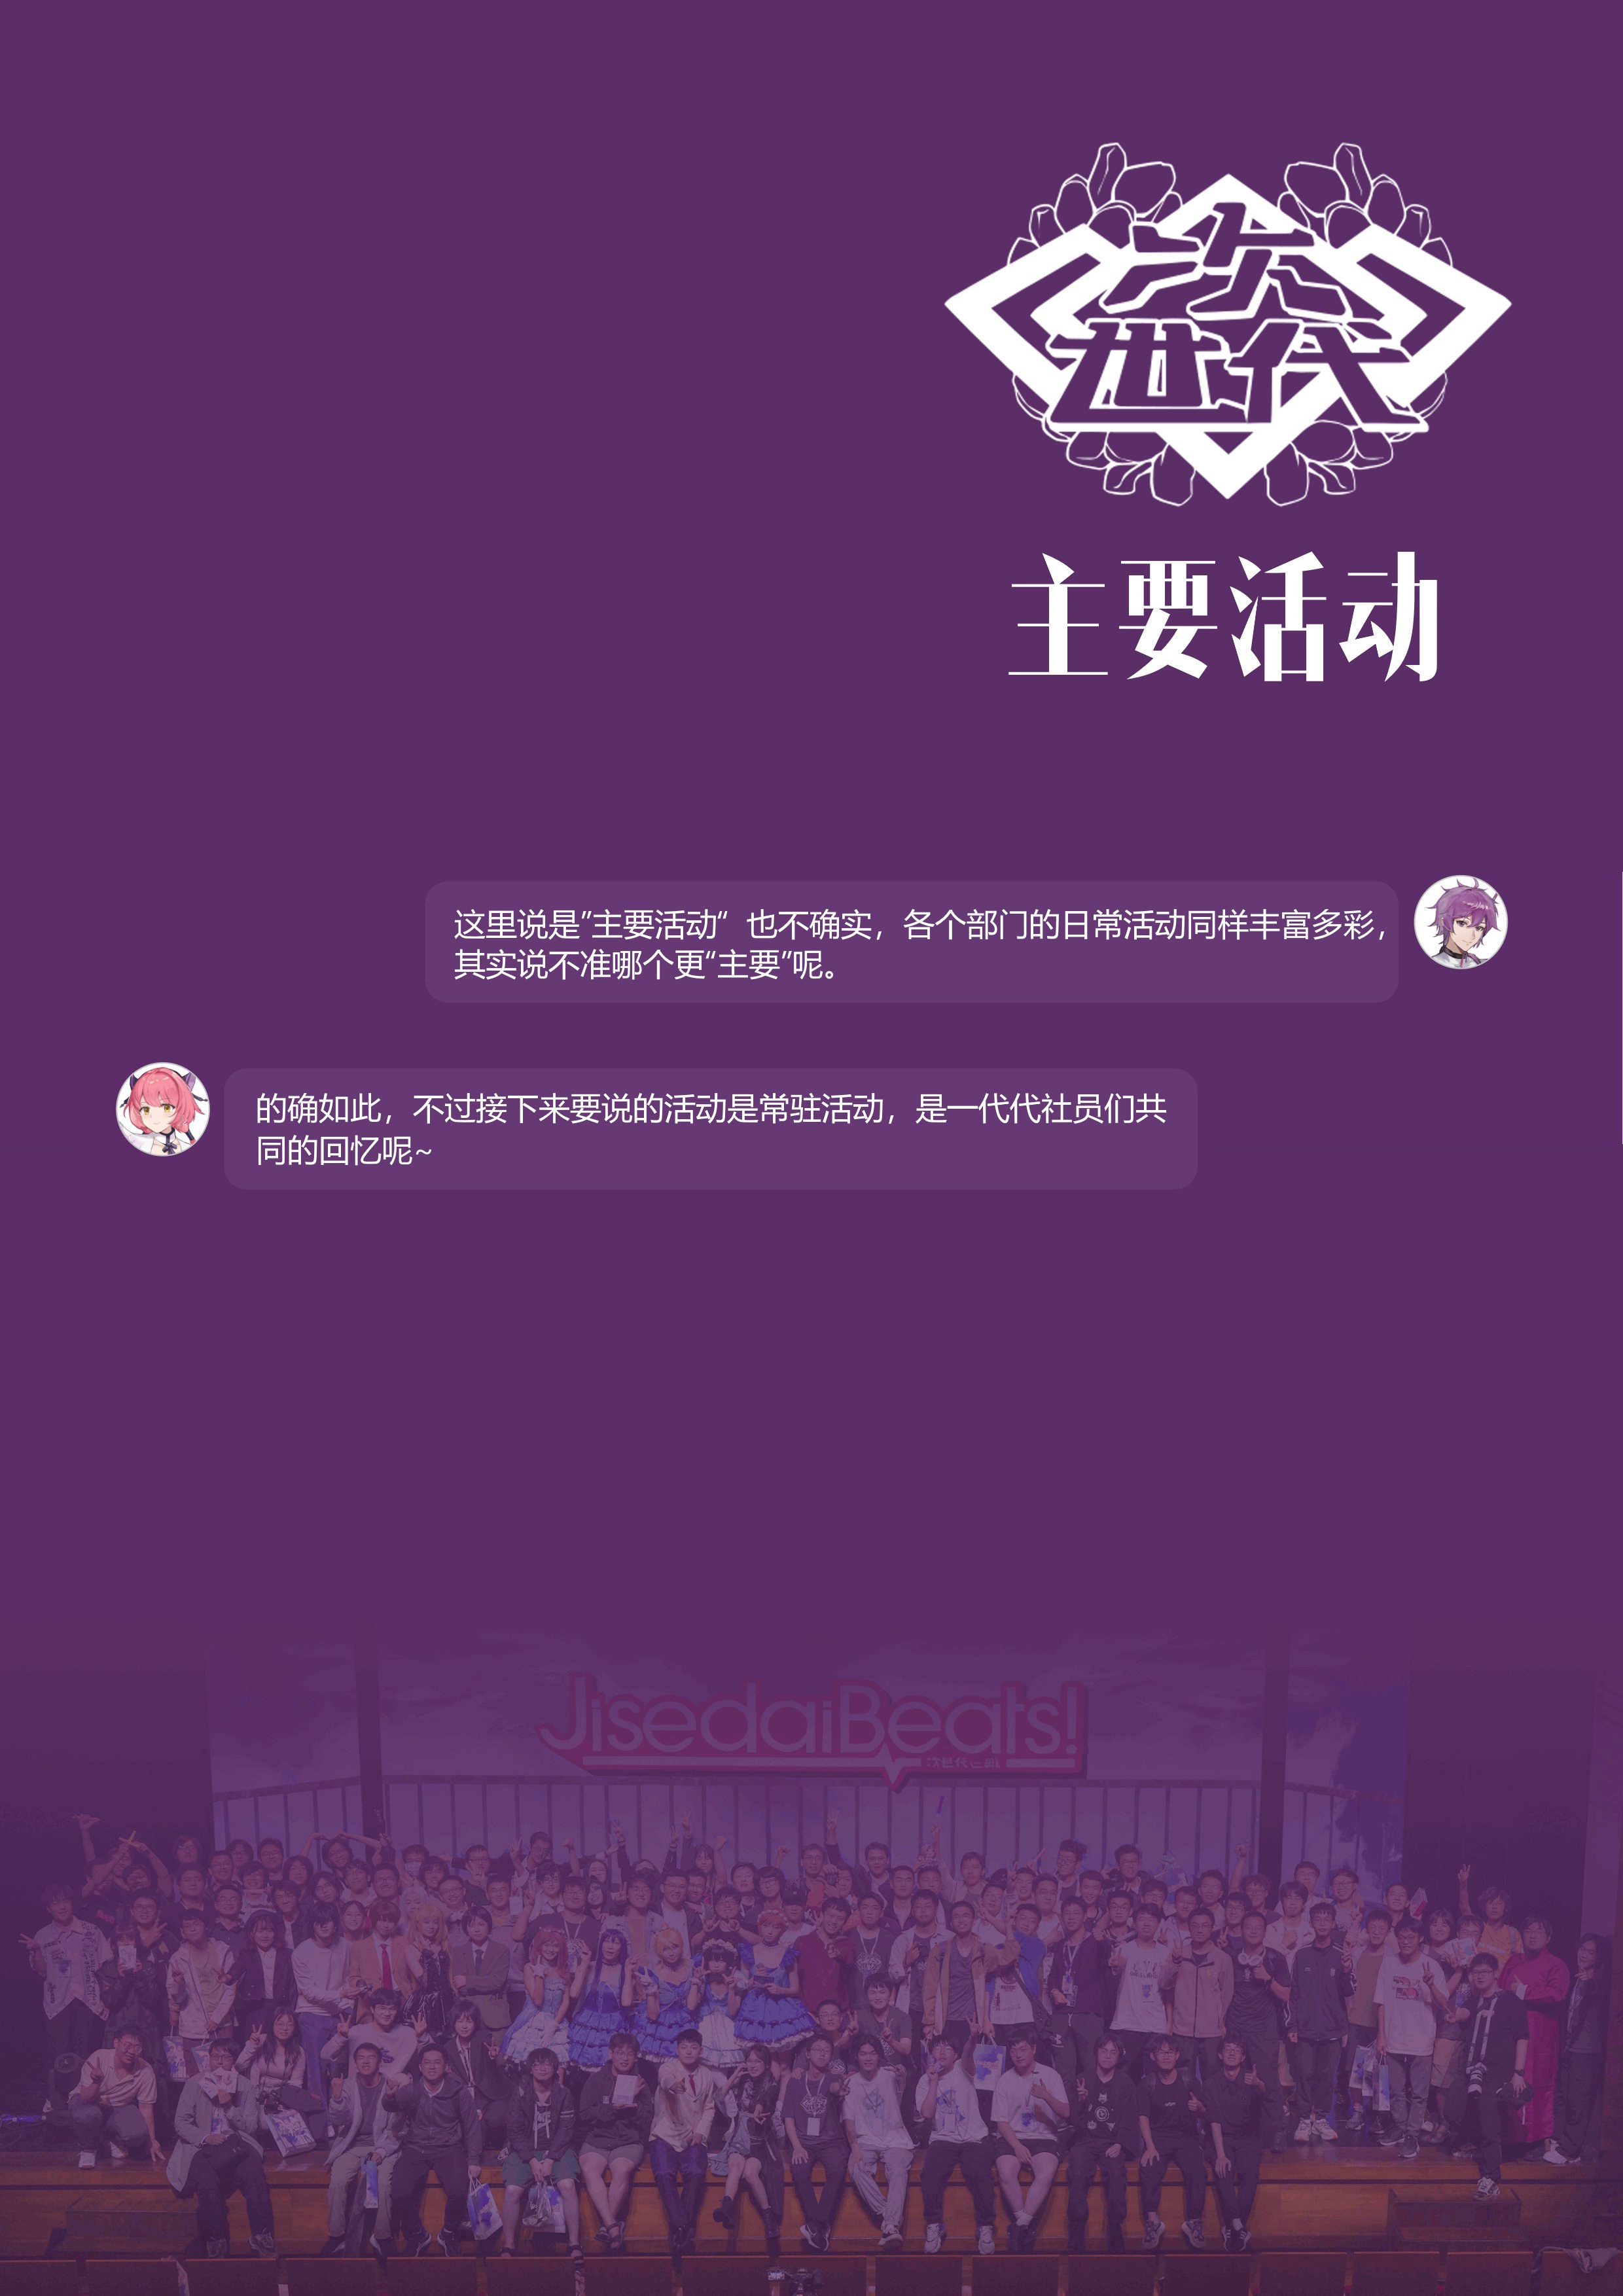
\includegraphics[width=0.9999\paperwidth, height=0.9999\paperheight]{ch2.jpg} % 插入图片,使其尺寸与纸张大小一致并保持宽高比[1](@ref)
    \restoregeometry % 恢复原来的页边距设置

\newpage
\newpage
\fontsize{23pt}{24pt}\selectfont
\begin{center}
    \textbf{\textcolor{truepurple}{百团大战\&迎新晚会}}\\
\end{center}
\vspace{0.7em}
\adjustbox{valign=t}{
	\begin{minipage}[t]{0.45\textwidth}
		\normalsize
		\chind 一年两度,次世代的大家拿出自己最大的热情欢迎新朋友!\\
    \chind 我们一直是百团最热闹的摊位之一。有各位同学自发贡献展示的手办、周边、图书展出;来自绘画部画师们的现场签绘、互绘;乐队部带来的现场演奏;cosplay舞台剧部的coser聚会、宅舞部献上的随舞表演;以及随后的wota艺节目……是招新,也是借机团建!\\
    \chind 在百团之后,我们会举办迎新晚会,进行各个分部的介绍展示与好玩的一站到底环节。\\
  		\par
		\vspace{-1em}
		\raisebox{-\height}{
			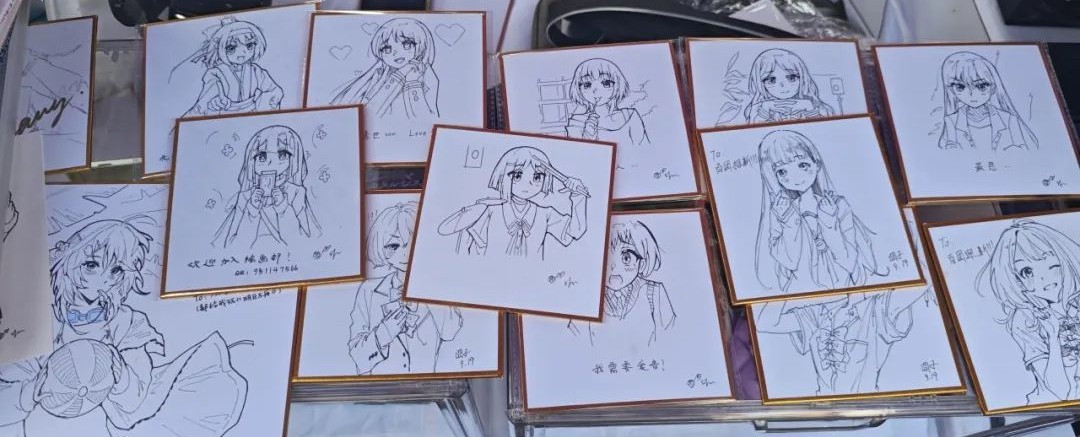
\includegraphics[width=\linewidth]{百团4.jpg}}
		\vspace{-0.5em}
		\picbox{\small ~\ding{115} ~ 绘画部现场签绘~}
		\par
		\vspace{-1em}
		\raisebox{-\height}{
			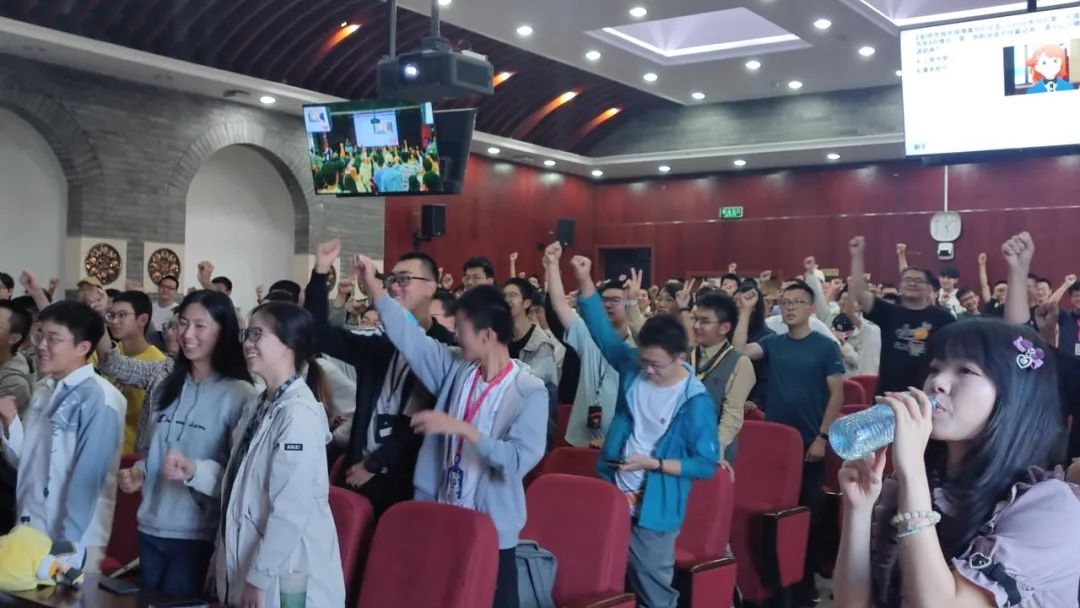
\includegraphics[width=\linewidth]{百团3.jpg}}
		\vspace{-0.5em}
		\picbox{\small ~\ding{115} ~ 一站到底~}
	\end{minipage}}
\hfill
\vspace{1em}
\adjustbox{valign=t}{
	\begin{minipage}[t]{0.45\textwidth}
		\vspace{-0.5em}
		\raisebox{-\height}{
			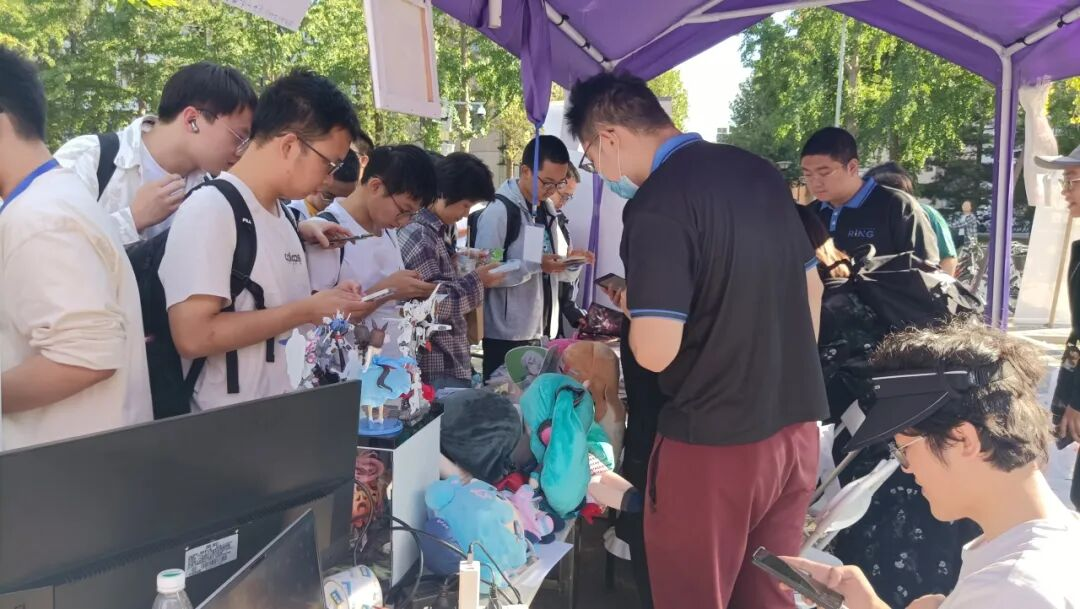
\includegraphics[width=\linewidth]{百团1.jpg}}
		\vspace{-0.5em}
		\picbox{\small ~\ding{115} ~ 走\scriptsize\sout{错}\normalsize\textbf{对}大学第一步~}
		\par
		\vspace{-1em}
		\raisebox{-\height}{
			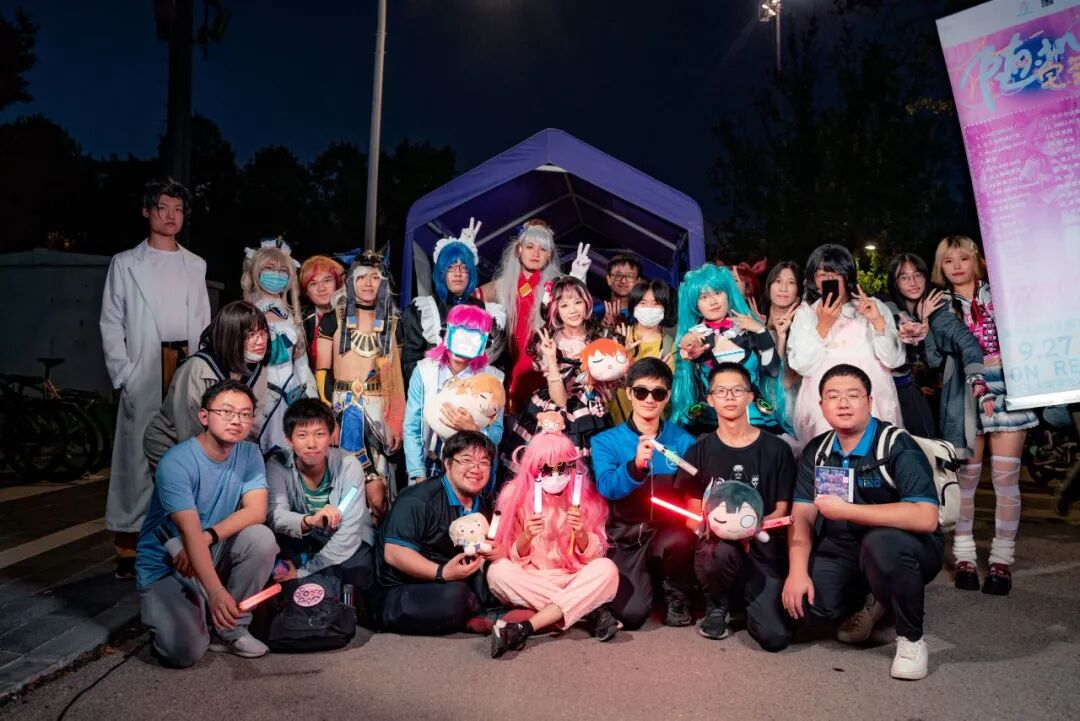
\includegraphics[width=\linewidth]{百团2.jpg}}
		\vspace{-0.5em}
		\picbox{\small ~\ding{115} ~ 随机宅舞~}
		\par
		\vspace{-1em}
		\raisebox{-\height}{
			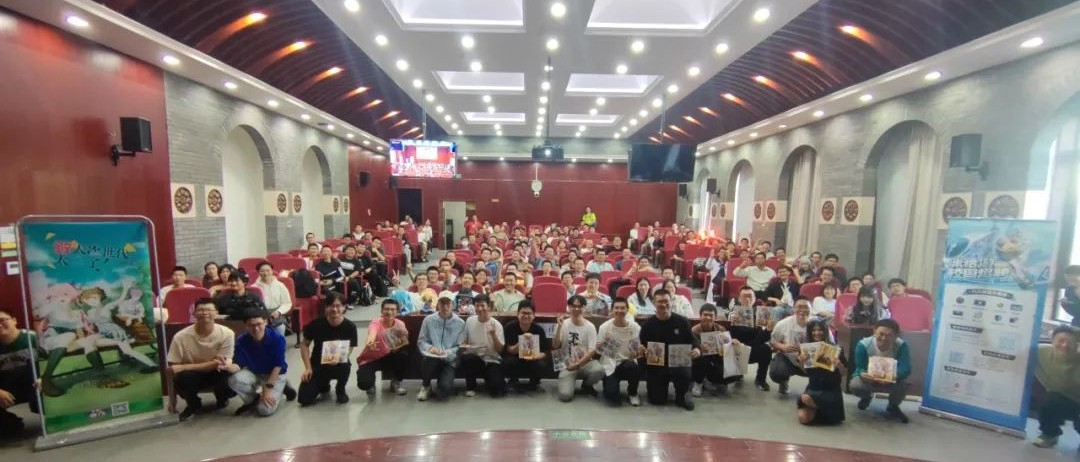
\includegraphics[width=\linewidth]{百团5.jpg}}
		\vspace{-0.5em}
		\picbox{\small ~\ding{115} ~ 迎新晚会合影~}
	\end{minipage}%
}
\begin{textblock*}{\paperwidth}(0mm, \dimexpr\paperheight-78.5mm\relax) % 距顶部 = 纸高 - 30mm
  \noindent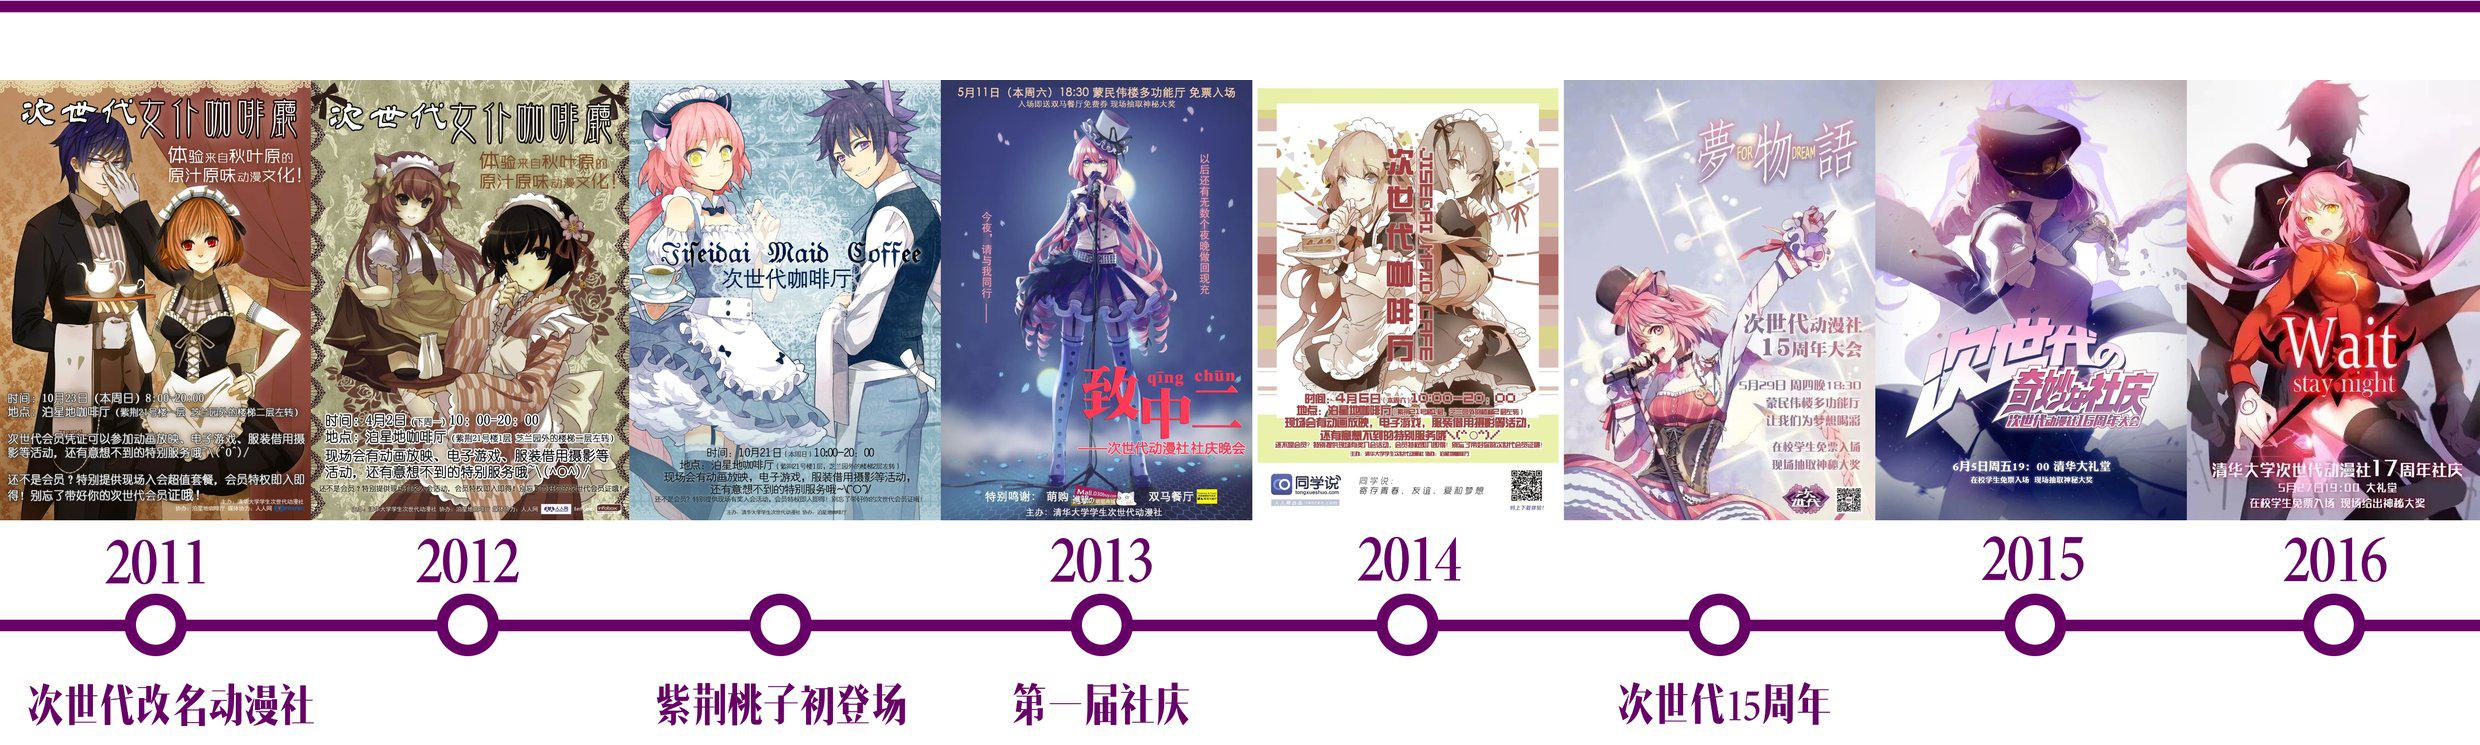
\includegraphics[width=\paperwidth]{tl1.jpg}
\end{textblock*}



\newpage
\fontsize{23pt}{24pt}\selectfont
\begin{center}
    \textbf{\textcolor{truepurple}{动漫主题咖啡厅}}\\
\end{center}
\vspace{0.7em}
\adjustbox{valign=t}{
	\begin{minipage}[t]{0.45\textwidth}
		\vspace{-0.5em}
		\raisebox{-\height}{
			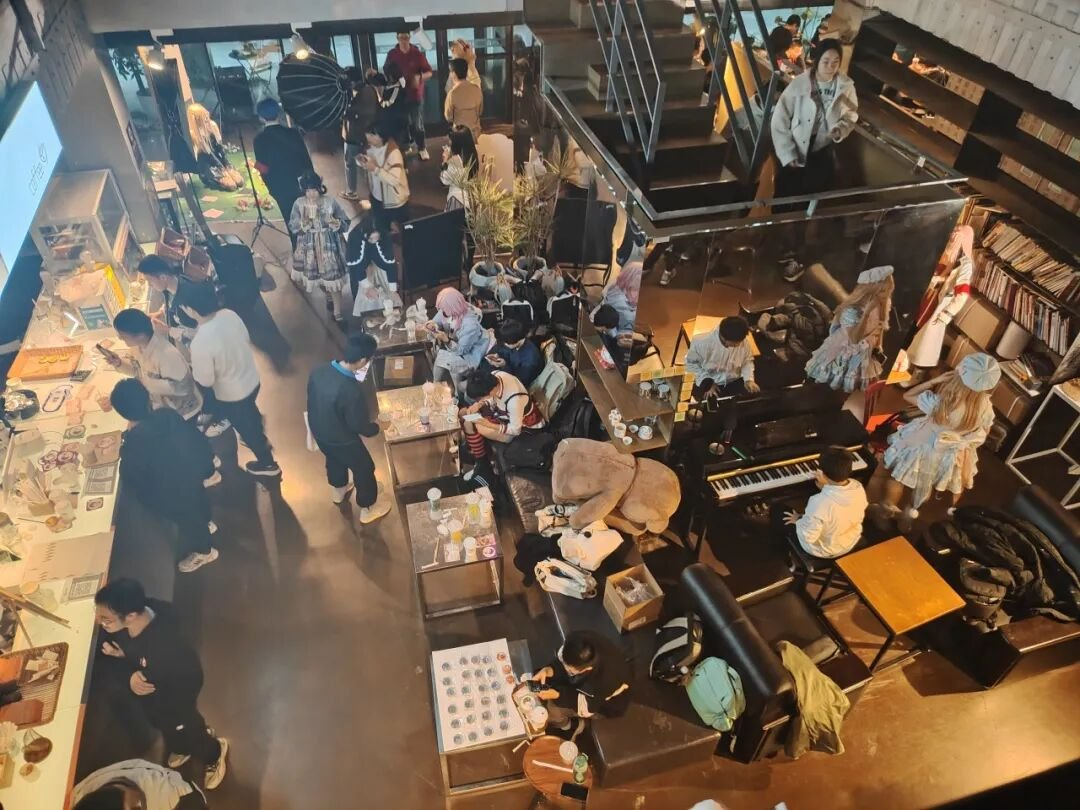
\includegraphics[width=0.9\linewidth]{咖啡厅3.jpg}}
		\vspace{-0.5em}
		\picbox{\small ~\ding{115} ~ 咖啡厅全景~}
  		\par
		\vspace{-1em}
		\raisebox{-\height}{
			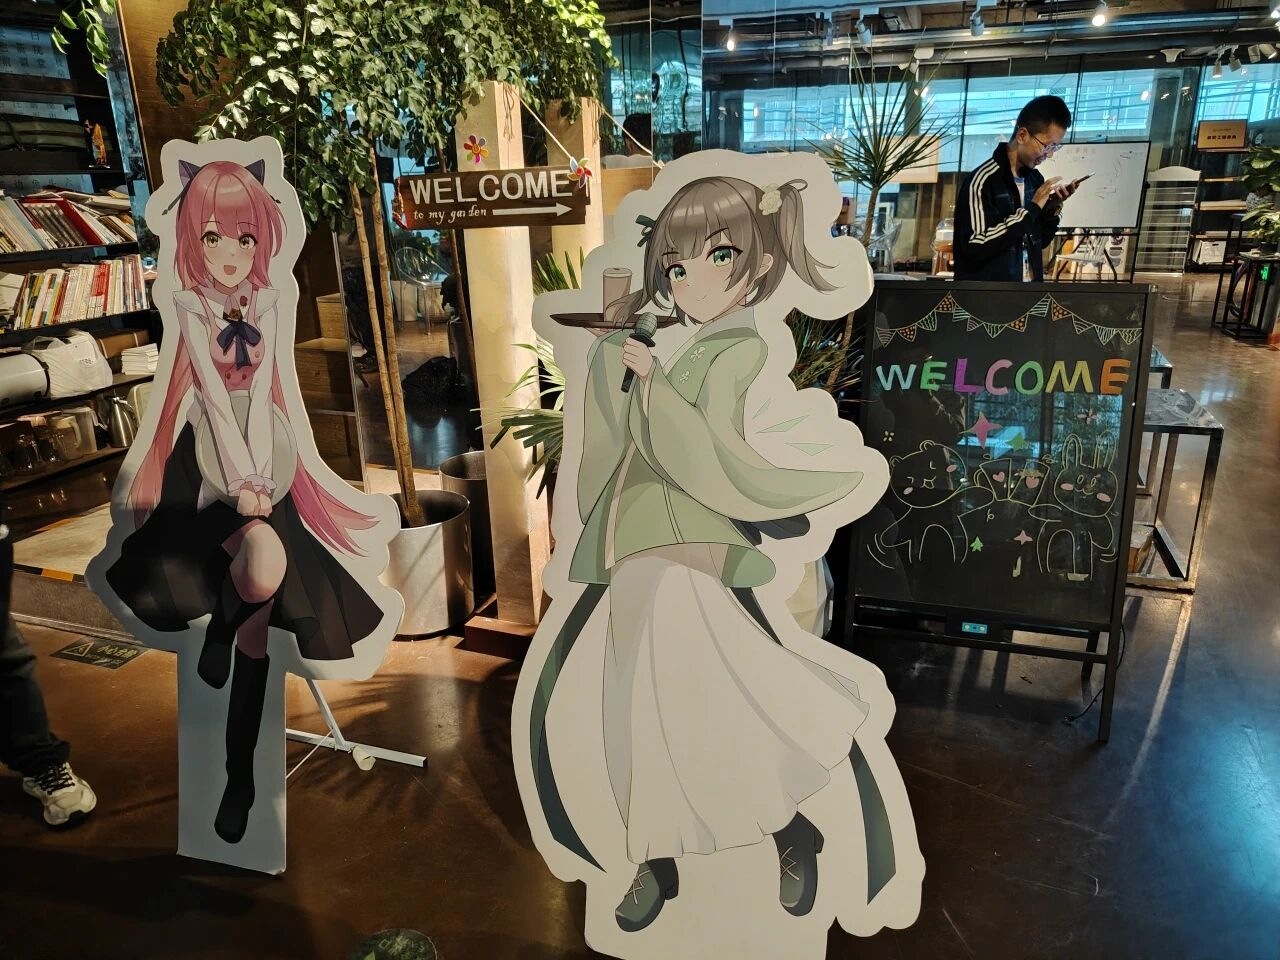
\includegraphics[width=0.9\linewidth]{咖啡厅2.jpg}}
		\vspace{-0.5em}
		\picbox{\small ~\ding{115} ~ 看板营业中~}
		\par
		\vspace{-1em}
		\raisebox{-\height}{
			\includegraphics[width=0.9\linewidth]{咖啡厅1.jpg}}
		\vspace{-0.5em}
		\picbox{\small ~\ding{115} ~ coser合影~}
	\end{minipage}}
\hfill
\vspace{1em}
\adjustbox{valign=t}{
	\begin{minipage}[t]{0.45\textwidth}

		\par
    \vspace{-0.5em}
		\raisebox{-\height}{
			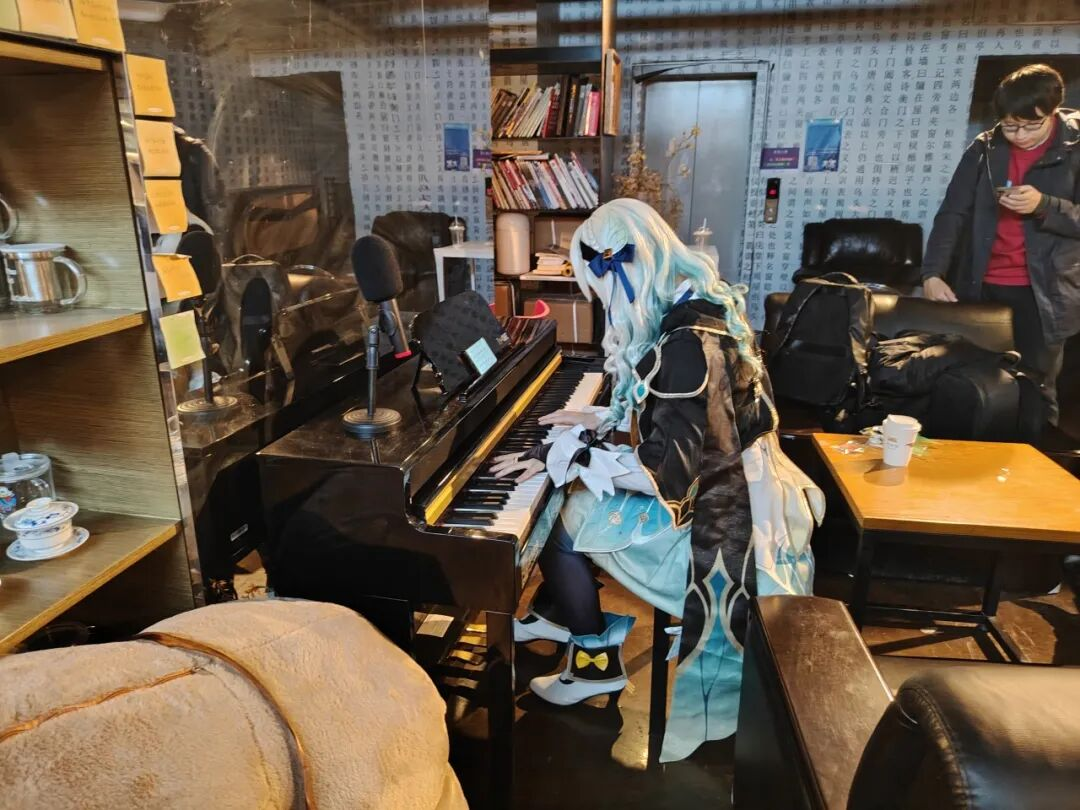
\includegraphics[width=0.9\linewidth]{咖啡厅4.jpg}}
		\vspace{-0.5em}
		\picbox{\small ~\ding{115} ~ 高雅的演奏家~}
		\normalsize
    \par
		\chind 动漫咖啡厅是每学期一度的,历史最悠久的次世代特色活动。\\
\chind 咖啡厅的咖啡师和服务生均由社员担任,不仅会提供各式点心和饮品特调,而且有紧张刺激的新番毒奶大会、剧场版动画连续放送,以及桌游、动画歌牌等游戏互动,还会不定期有茶绘现场看哦。当然还有必不可少的抽奖环节.jpg\\
\chind 这里同时也是cosplay的绝妙场所、外社联动的常见平台。\\
		\par
		\vspace{-2em}
		\raisebox{-\height}{
			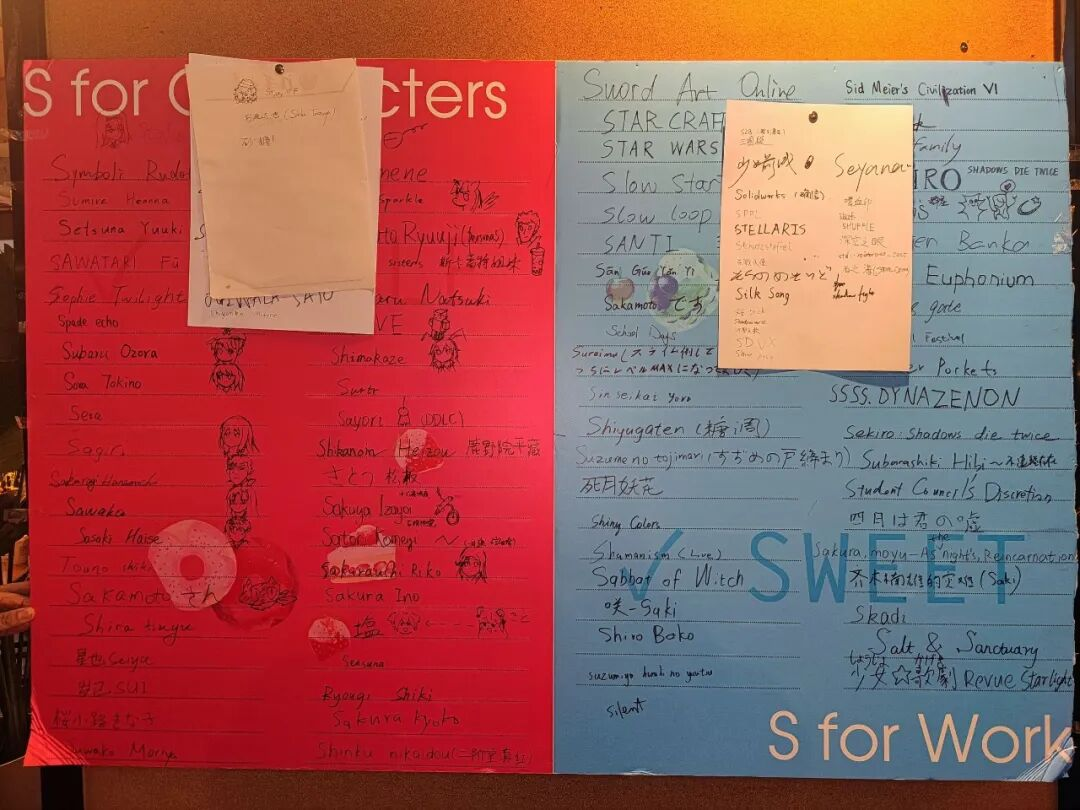
\includegraphics[width=0.8\linewidth]{咖啡厅5.jpg}}
		\vspace{-0.5em}
		\picbox{\small ~\ding{115} ~ S for what?~}

	\end{minipage}%
}
\begin{textblock*}{\paperwidth}(0mm, \dimexpr\paperheight-78.5mm\relax) % 距顶部 = 纸高 - 30mm
  \noindent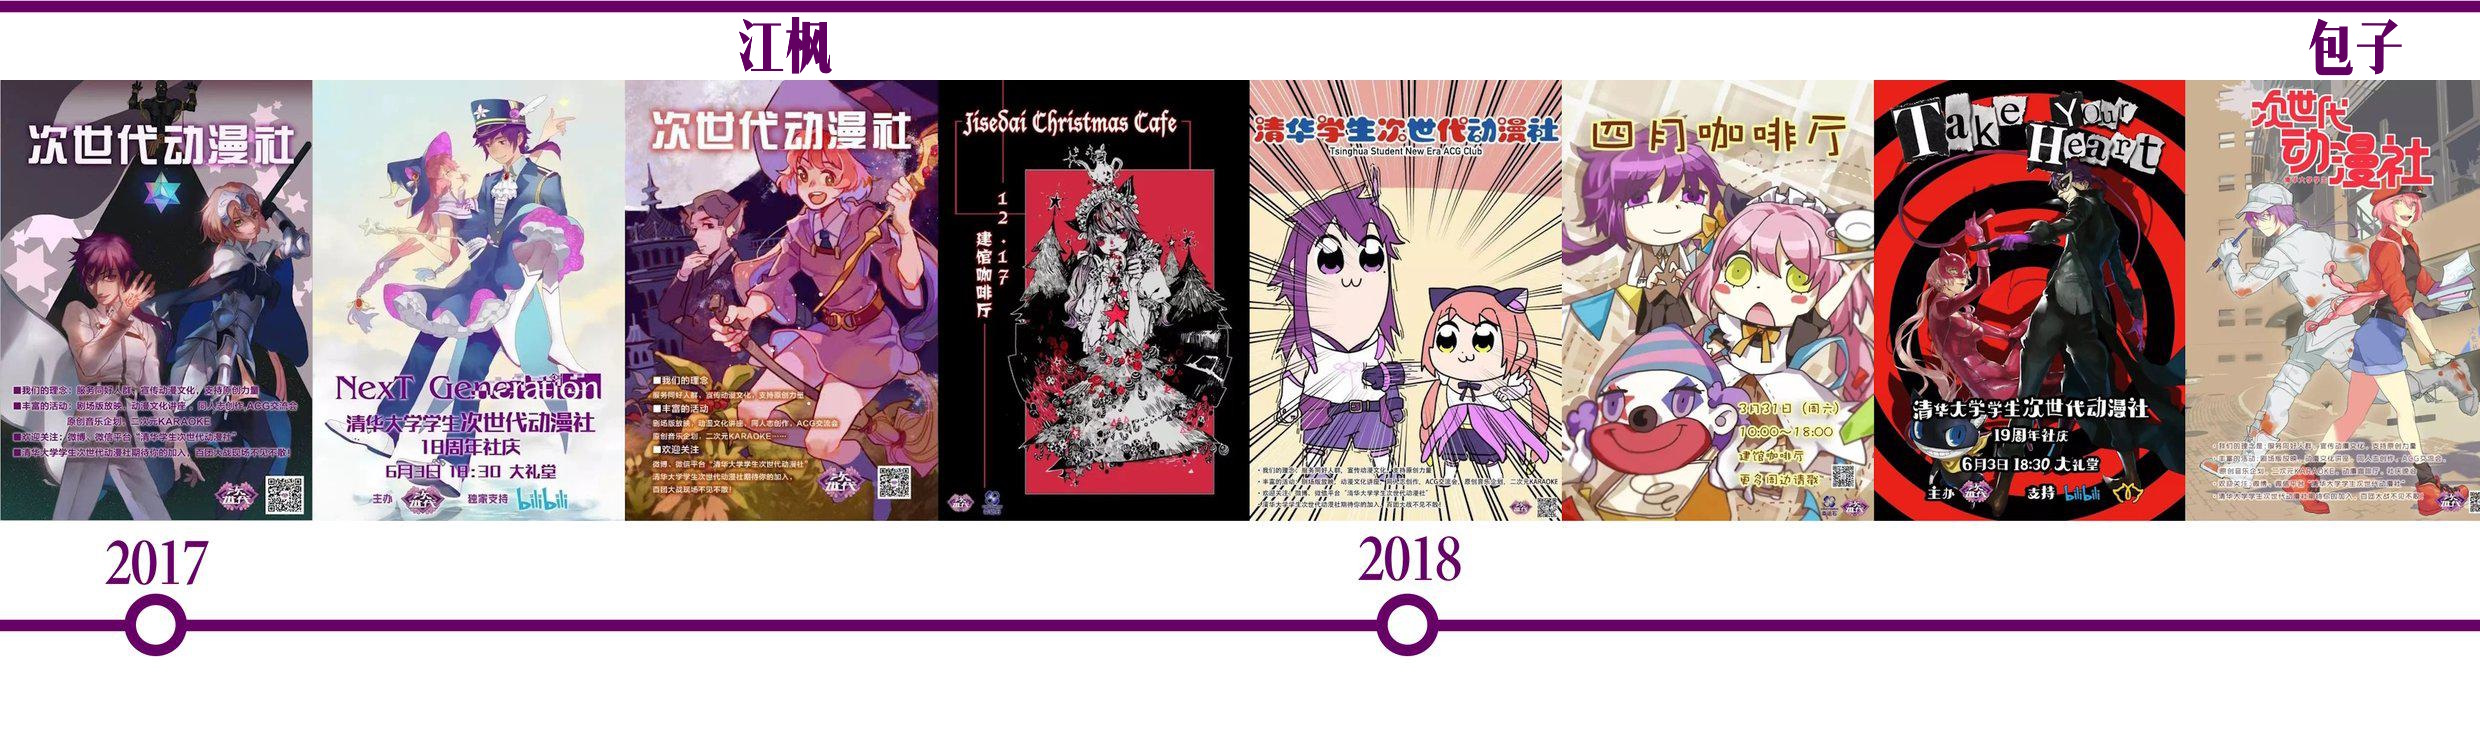
\includegraphics[width=\paperwidth]{tl2.jpg}
\end{textblock*}
\newpage
\fontsize{26pt}{28pt}\selectfont
\begin{center}
    \textbf{\textcolor{truepurple}{次世代社庆}}\\
\end{center}
\normalsize
\chind 一年一度由各兴趣部门共同精心打造,\textbf{与学生节同等规格的大型ACGN主题晚会}。目前已经举办了13届!\sout{(大型网友面基现场)}\\
\chind 如果你对一份属于你的二次元舞台有梦想,无论梦中的你是翩翩起舞的舞者还是激昂澎湃的乐手,是倾情演绎的演员还是引亢高歌的最强音,是聚光灯下的主持人还是幕后奉献的staff,所有的岗席与角色正虚位以待;\\
\chind 如果你只想坐在观众席欣赏表演,那么除了欣赏节目之外,也可以参与宅力大比拼的一站到底,抑或等待欧皇附体成为抽奖的幸运儿,当然无论如何都有三位看板的免费周边放送!\\
\chind 作为次世代最为盛大的年度活动,社庆为每一位心怀梦想的社友提供了施展才华的舞台。身为次世代社员的你怎能错过!\\
\vspace{1em}
\par
\adjustbox{valign=t}{
	\begin{minipage}[t]{0.45\textwidth}
		
		\raisebox{-\height}{
			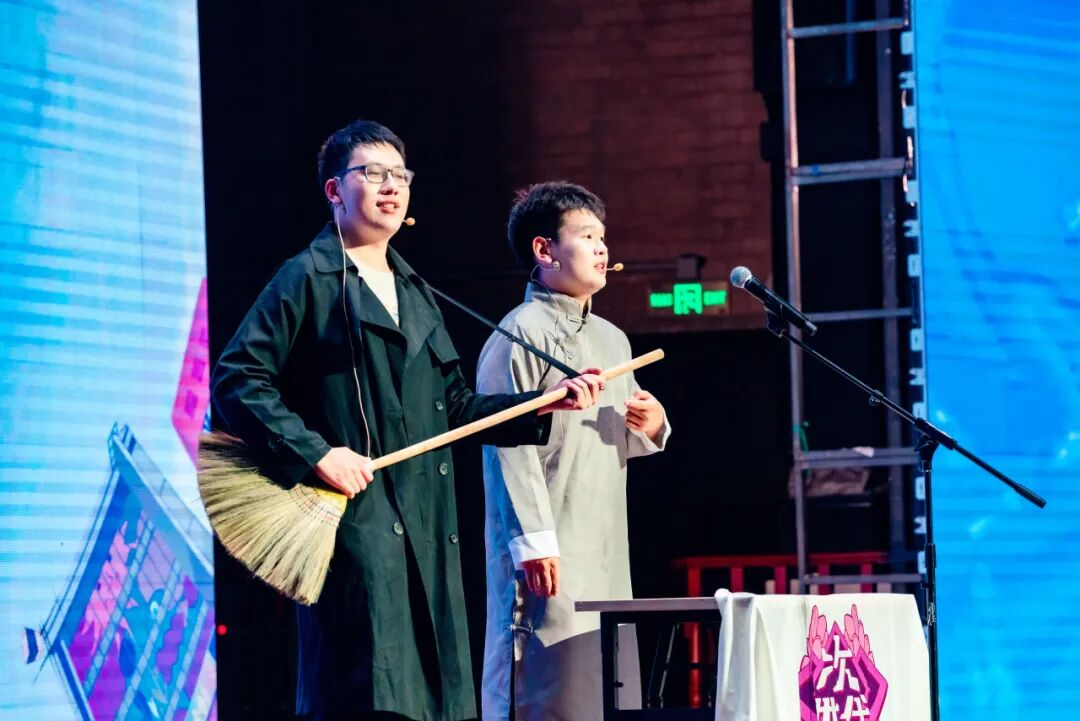
\includegraphics[width=0.9\linewidth]{社庆3.jpg}}
		\vspace{-0.5em}
		\picbox{\small \ding{115} 传世经典相声《我要玩乐队》}
  		\par
		\vspace{-0.5em}
		\raisebox{-\height}{
			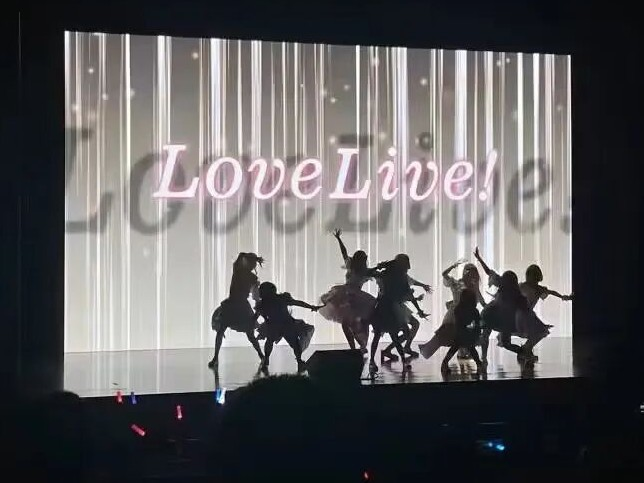
\includegraphics[width=0.9\linewidth]{社庆1.jpg}}
		\vspace{-0.5em}
		\picbox{\small ~\ding{115} ~ Lovelive!特别节目~}
	\end{minipage}}
\hfill
\vspace{1em}
\adjustbox{valign=t}{
	\begin{minipage}[t]{0.45\textwidth}
		\par
    
		\raisebox{-\height}{
			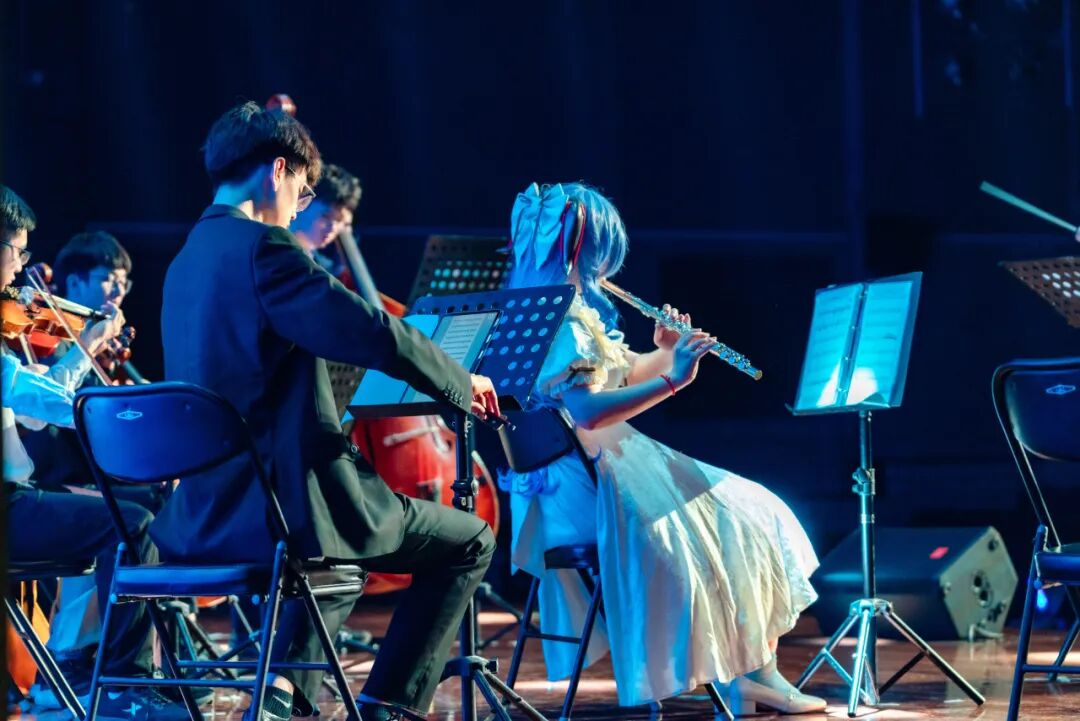
\includegraphics[width=0.9\linewidth]{社庆4.jpg}}
		\vspace{-0.5em}
		\picbox{\small ~\ding{115} ~ 室内乐节目~}
		\normalsize
    \par
		\vspace{0.5em}
		\raisebox{-\height}{
			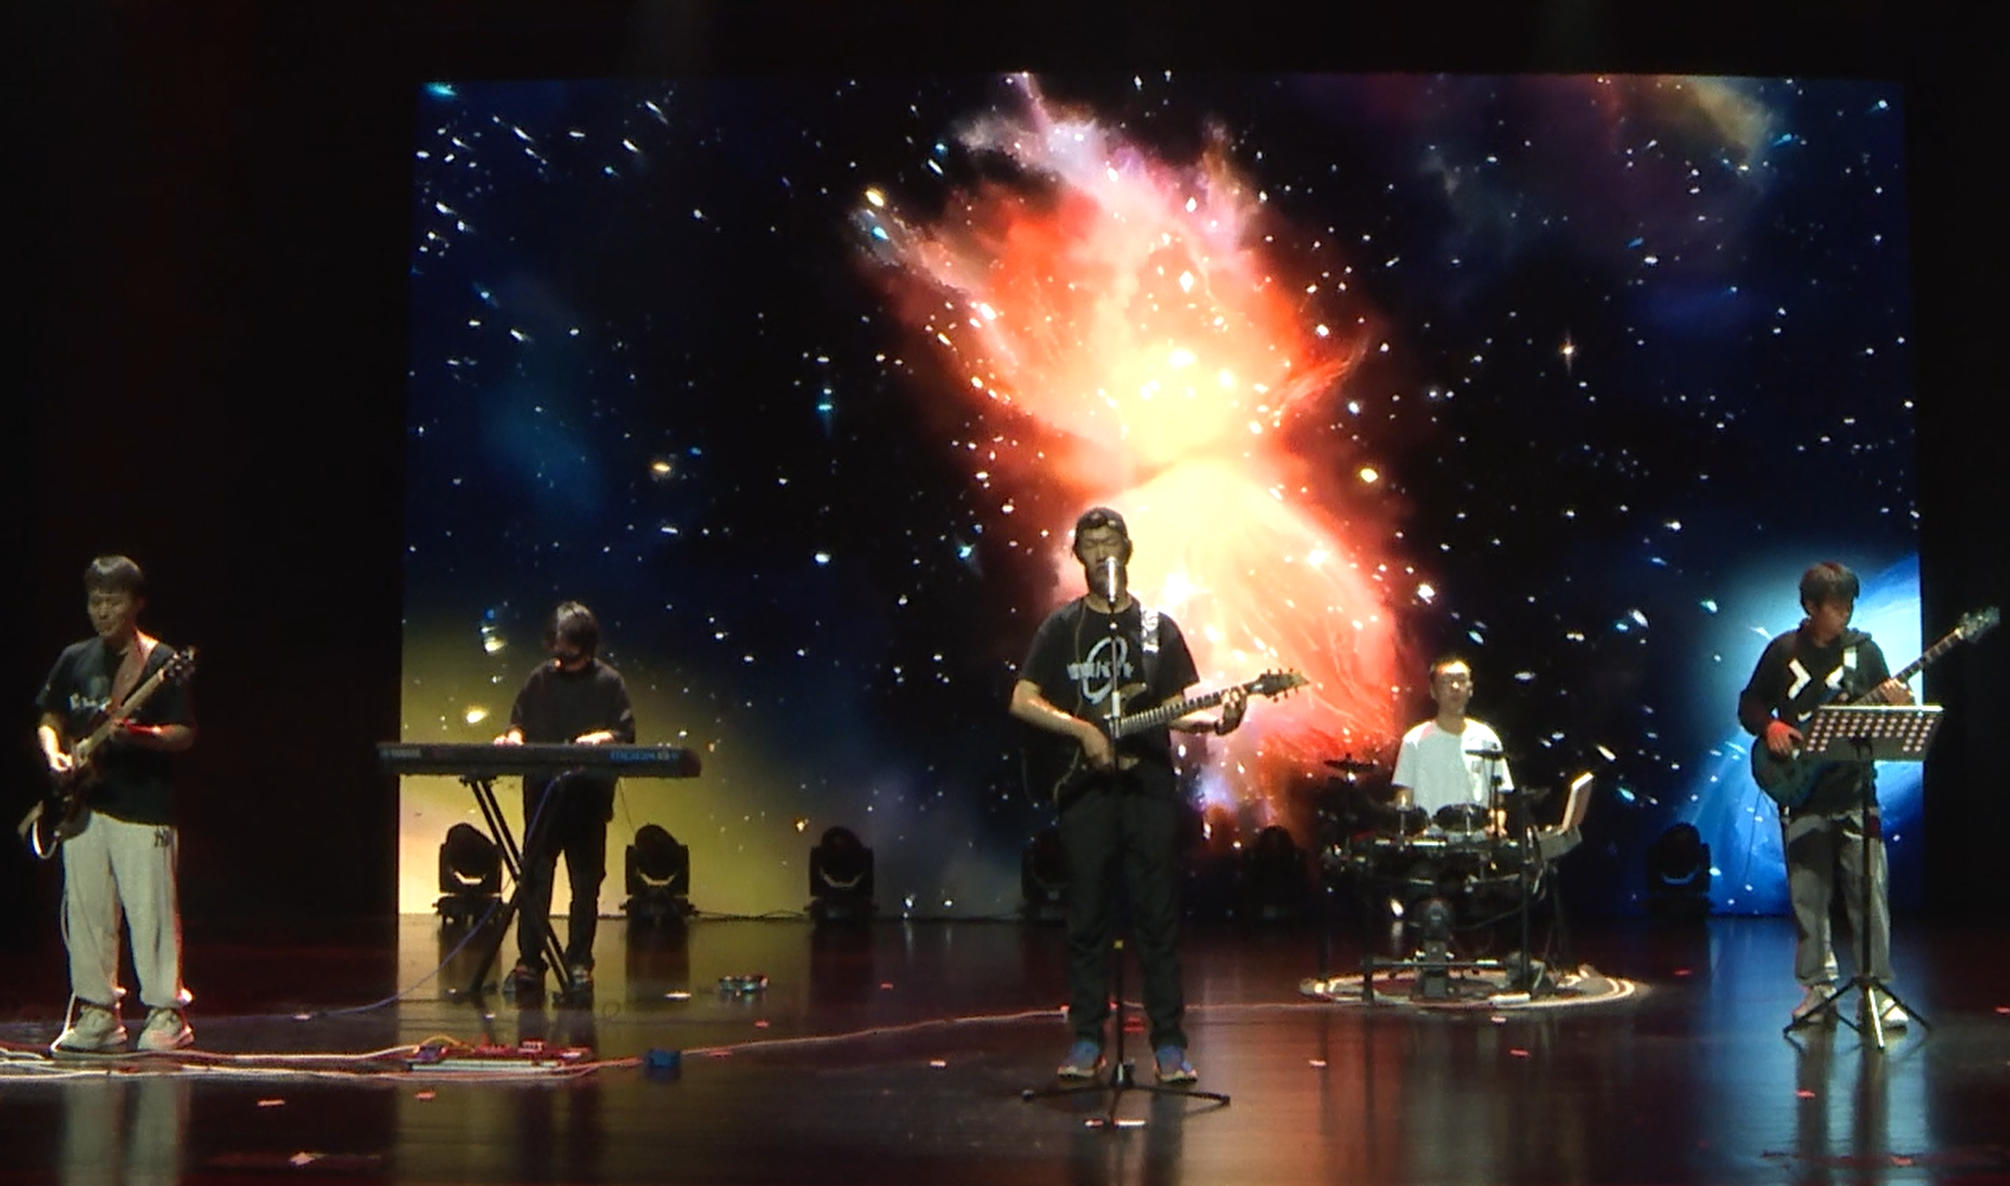
\includegraphics[width=0.9\linewidth]{社庆10.jpg}}
		\vspace{-0.5em}
		\picbox{\small ~\ding{115} ~ 乐队开场《再飞行》~}

	\end{minipage}%
}
\begin{textblock*}{\paperwidth}(0mm, \dimexpr\paperheight-78.5mm\relax) % 距顶部 = 纸高 - 30mm
  \noindent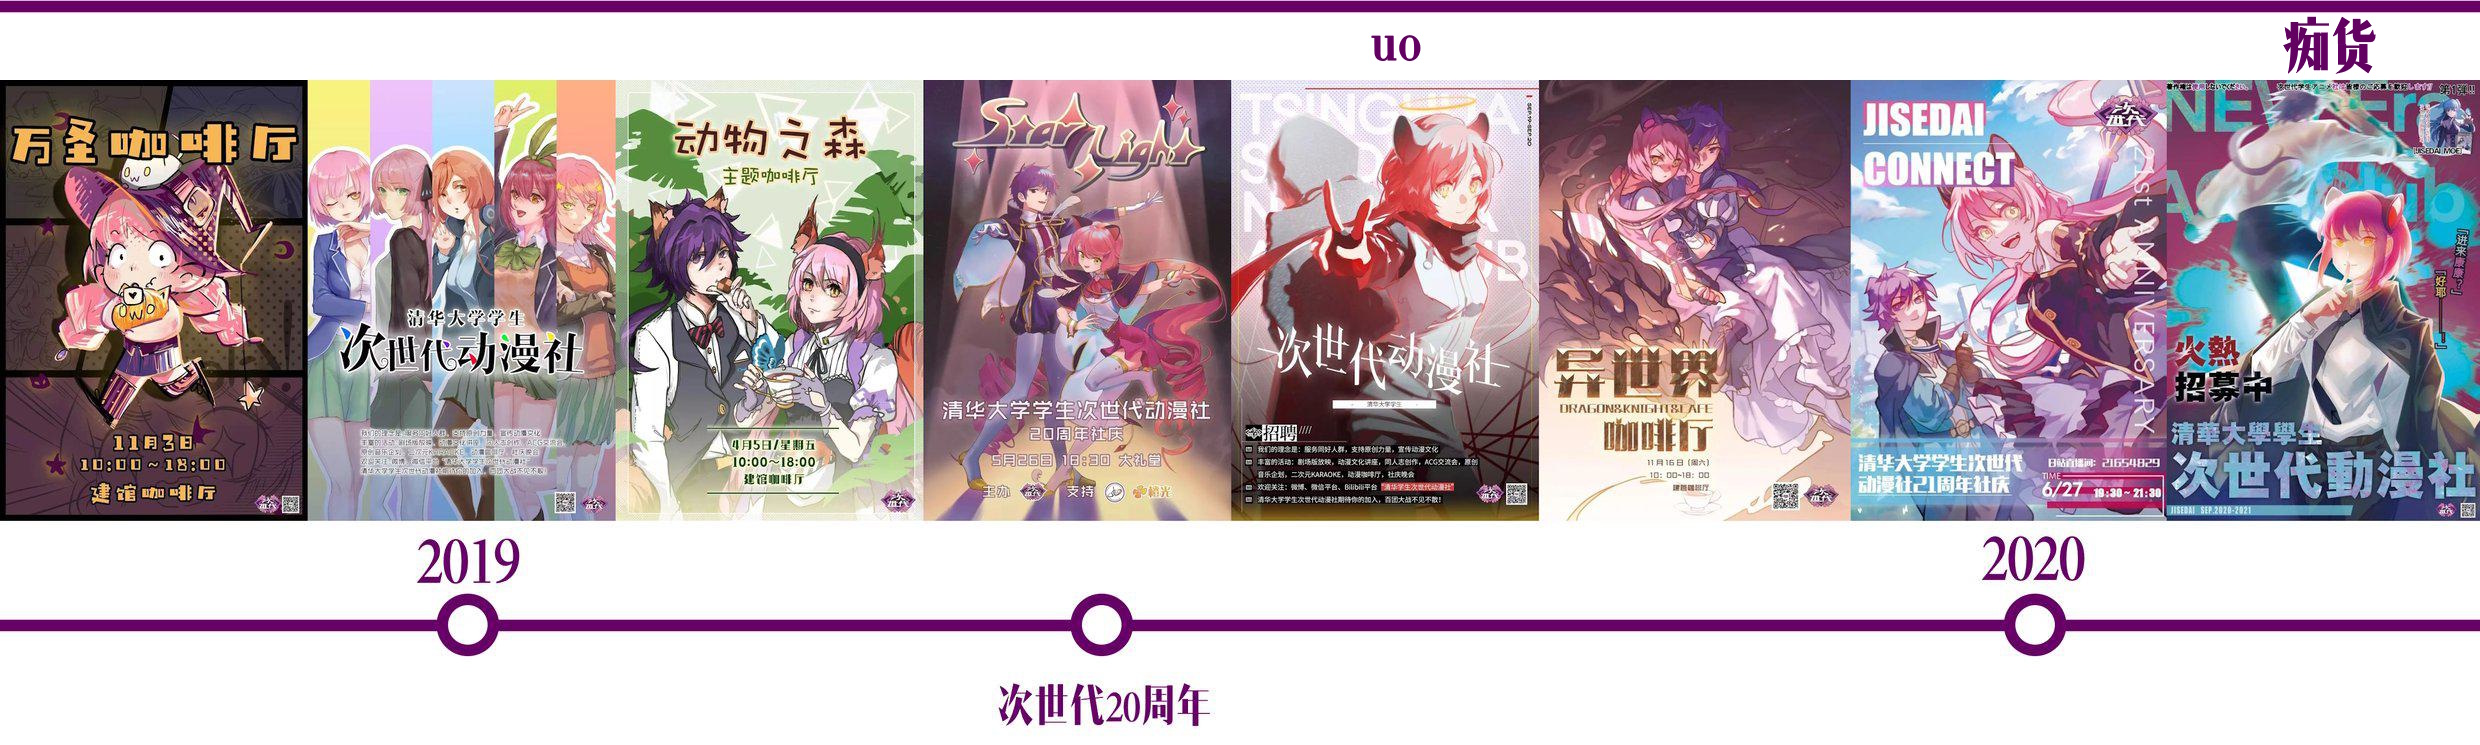
\includegraphics[width=\paperwidth]{tl3.jpg}
\end{textblock*}



\newpage
\par
\adjustbox{valign=t}{
	\begin{minipage}[t]{0.45\textwidth}
		
		\raisebox{-\height}{
			\includegraphics[width=0.9\linewidth]{社庆5.jpg}}
		\vspace{-0.5em}
		\picbox{\small \ding{115} 舞台剧《苹果默示录》}
  		\par
		\vspace{-0.5em}
		\raisebox{-\height}{
			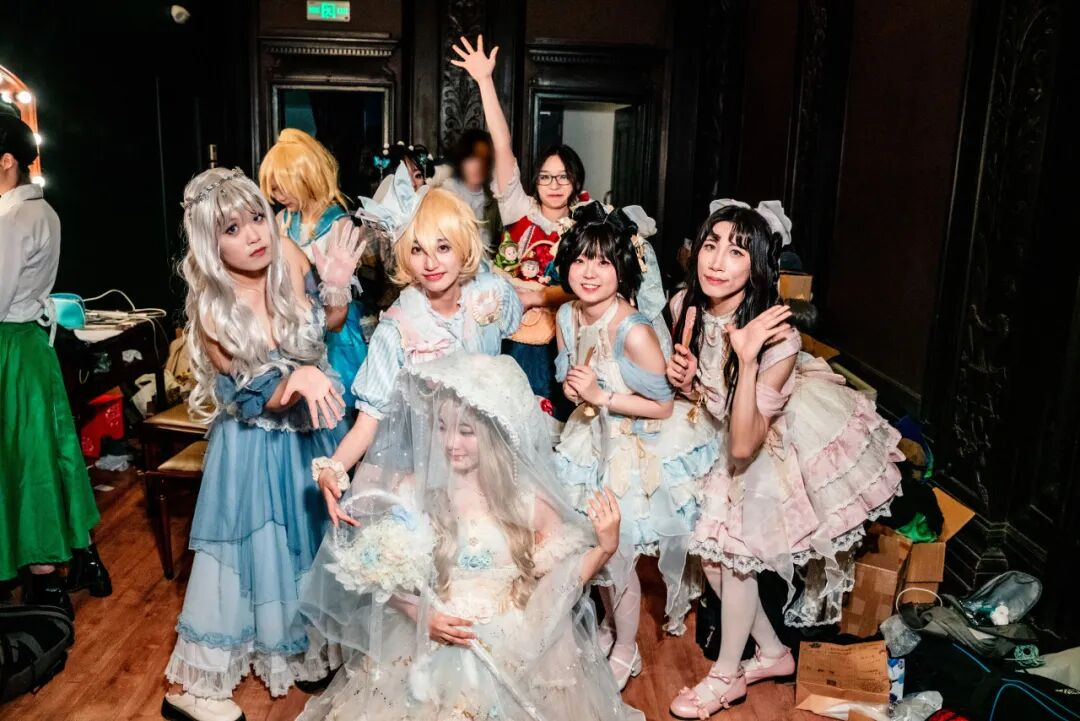
\includegraphics[width=0.9\linewidth]{社庆8.jpg}}
		\vspace{-0.5em}
		\picbox{\small ~\ding{115} ~ 在化妆间~}
	\end{minipage}}
\hfill
\vspace{1em}
\adjustbox{valign=t}{
	\begin{minipage}[t]{0.45\textwidth}
		\par
    
		\raisebox{-\height}{
			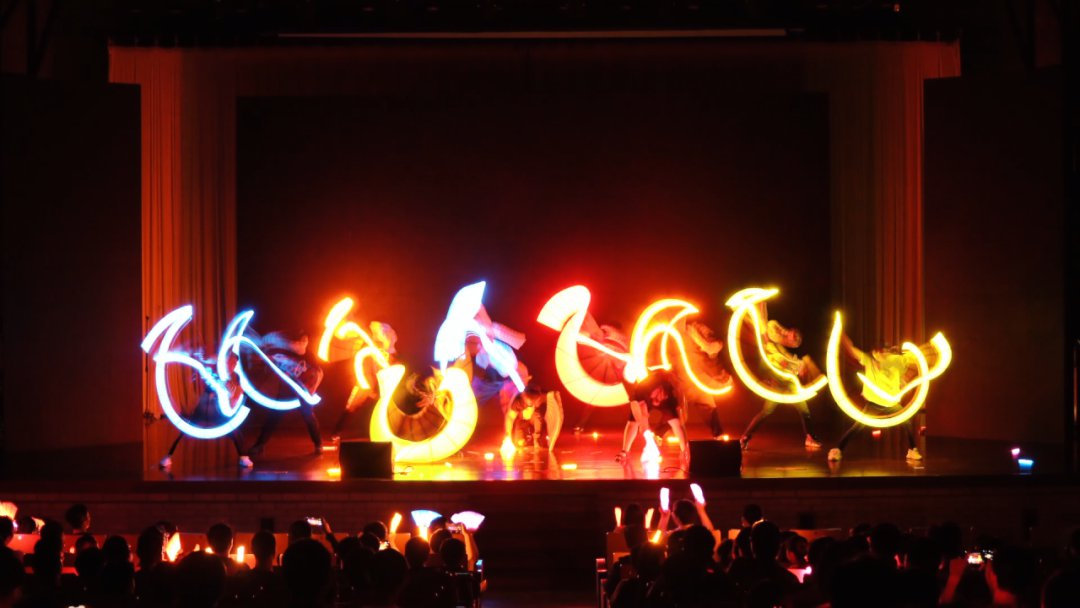
\includegraphics[width=0.9\linewidth]{社庆6.jpg}}
		\vspace{-0.5em}
		\picbox{\small ~\ding{115} ~ WOTA艺节目~}
		\normalsize
    \par
		\vspace{1.5em}
		\raisebox{-\height}{
			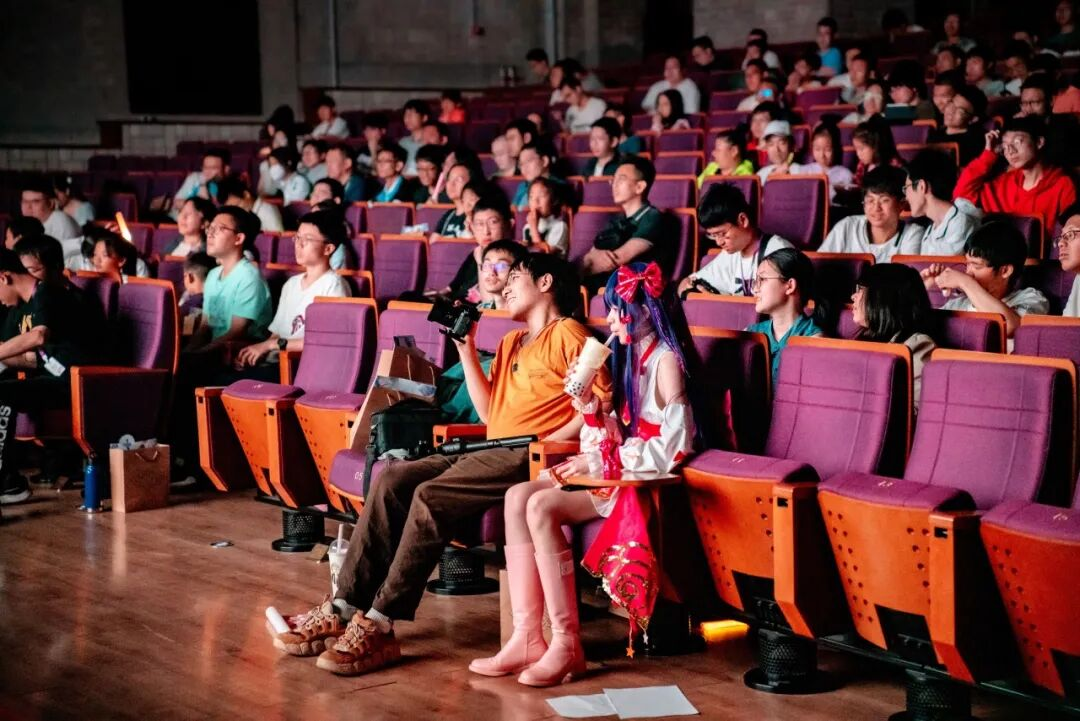
\includegraphics[width=0.9\linewidth]{社庆9.jpg}}
		\vspace{-0.5em}
		\picbox{\small ~\ding{115} ~ 溢出舞台的喜悦~}

	\end{minipage}%
}
\begin{center}
		\raisebox{-\height}{
			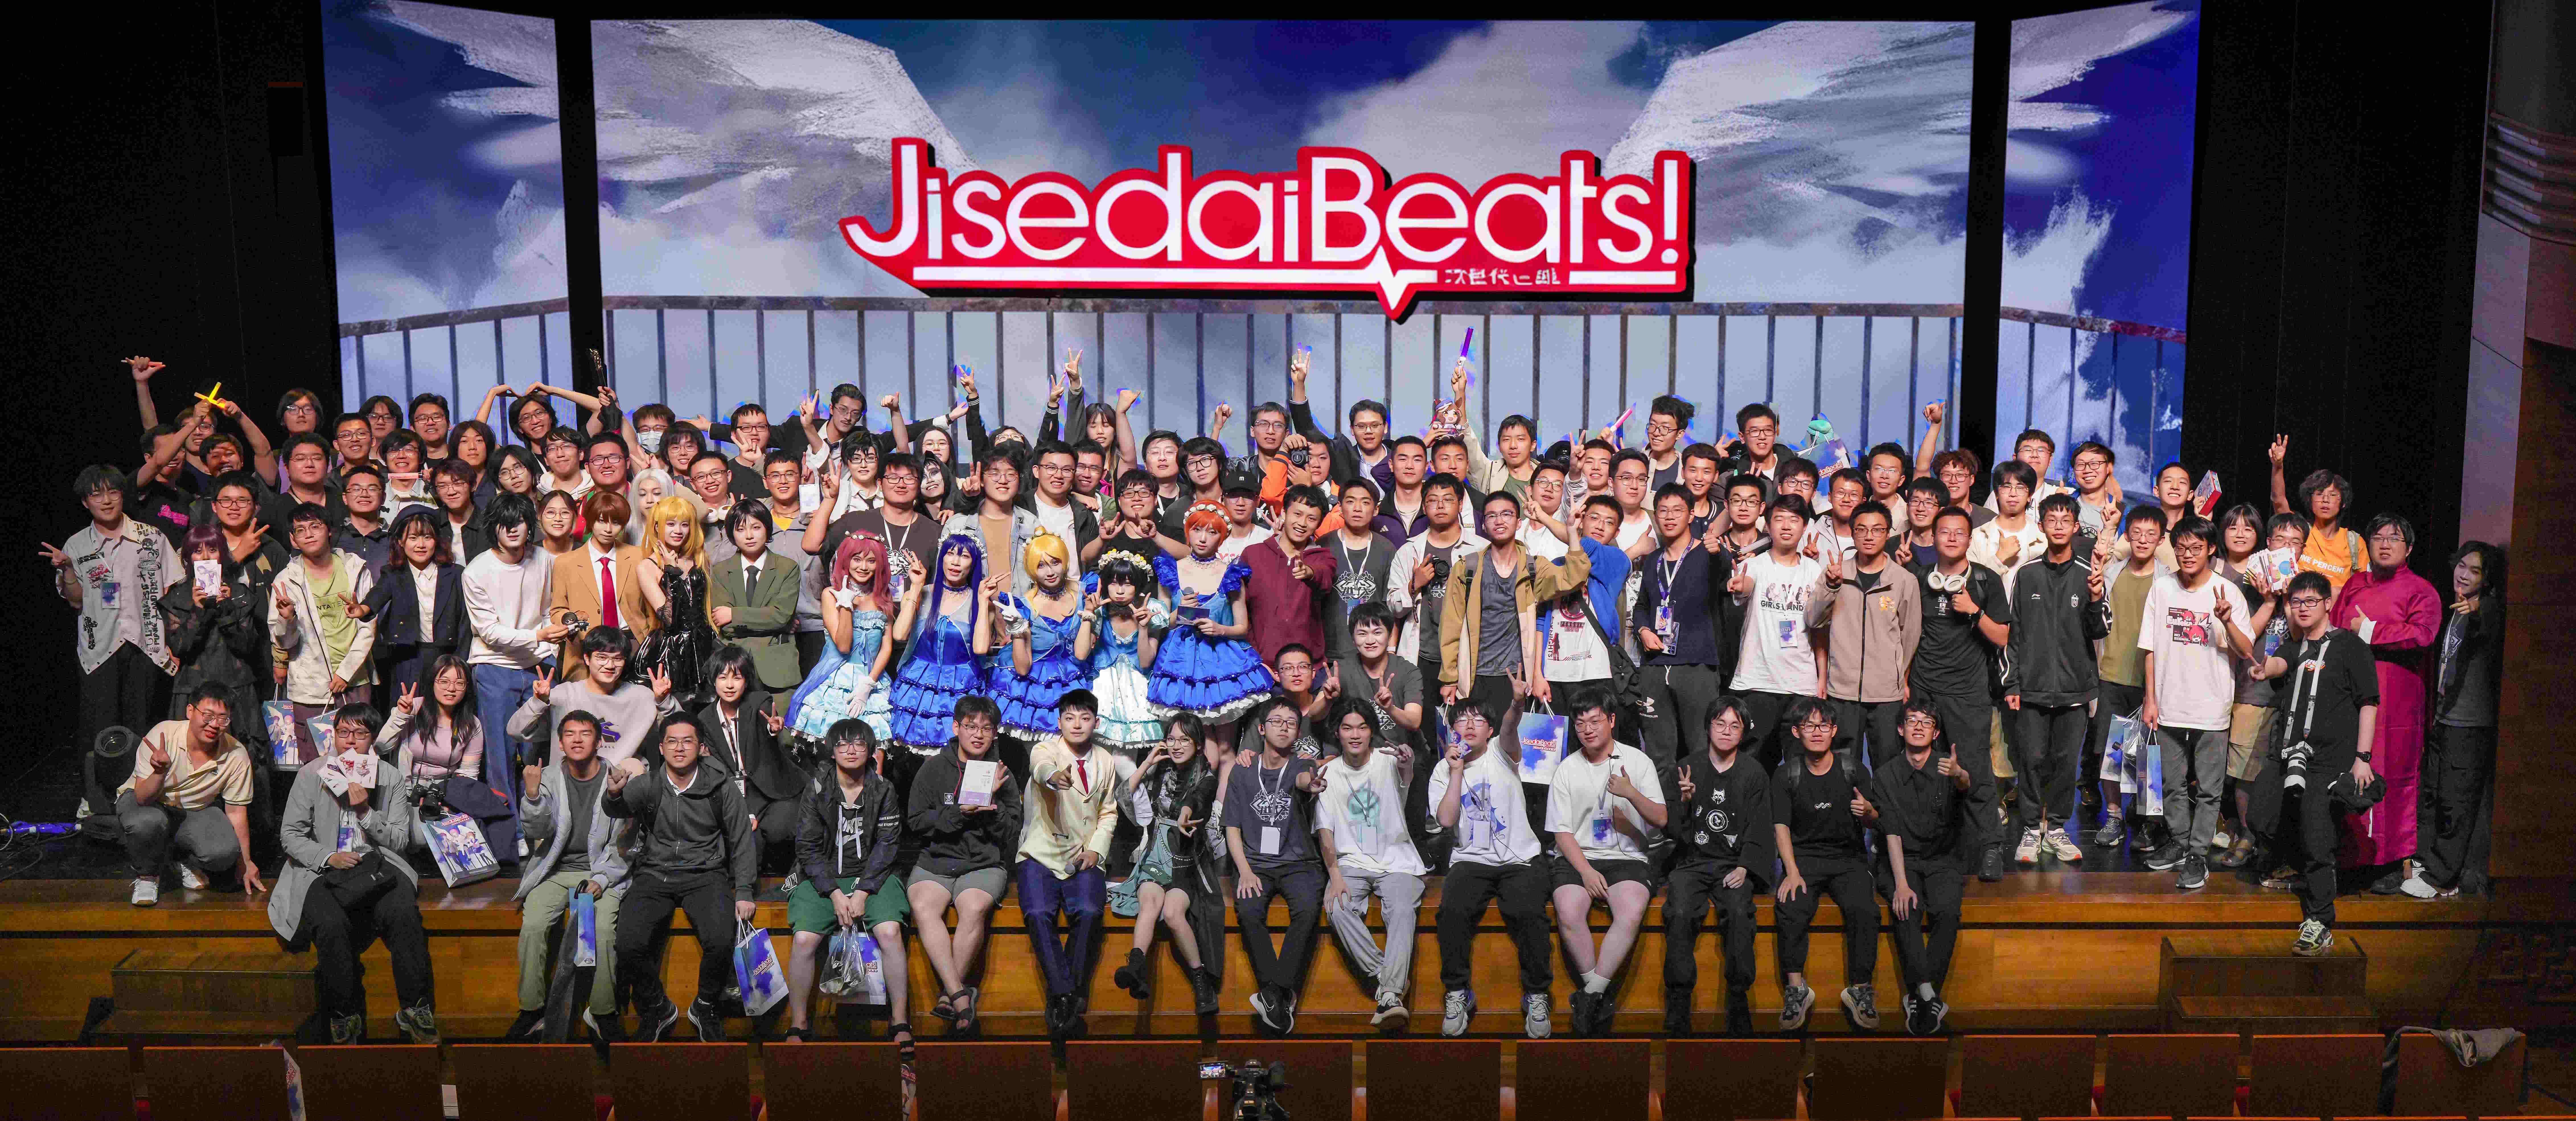
\includegraphics[width=0.9\linewidth]{社庆7.jpeg}}
		\vspace{-0.5em}
		\picbox{\small ~\ding{115} ~ 2025社庆~JisedaiBeats~大合照~}
\end{center}
\begin{textblock*}{\paperwidth}(0mm, \dimexpr\paperheight-78.5mm\relax) % 距顶部 = 纸高 - 30mm
  \noindent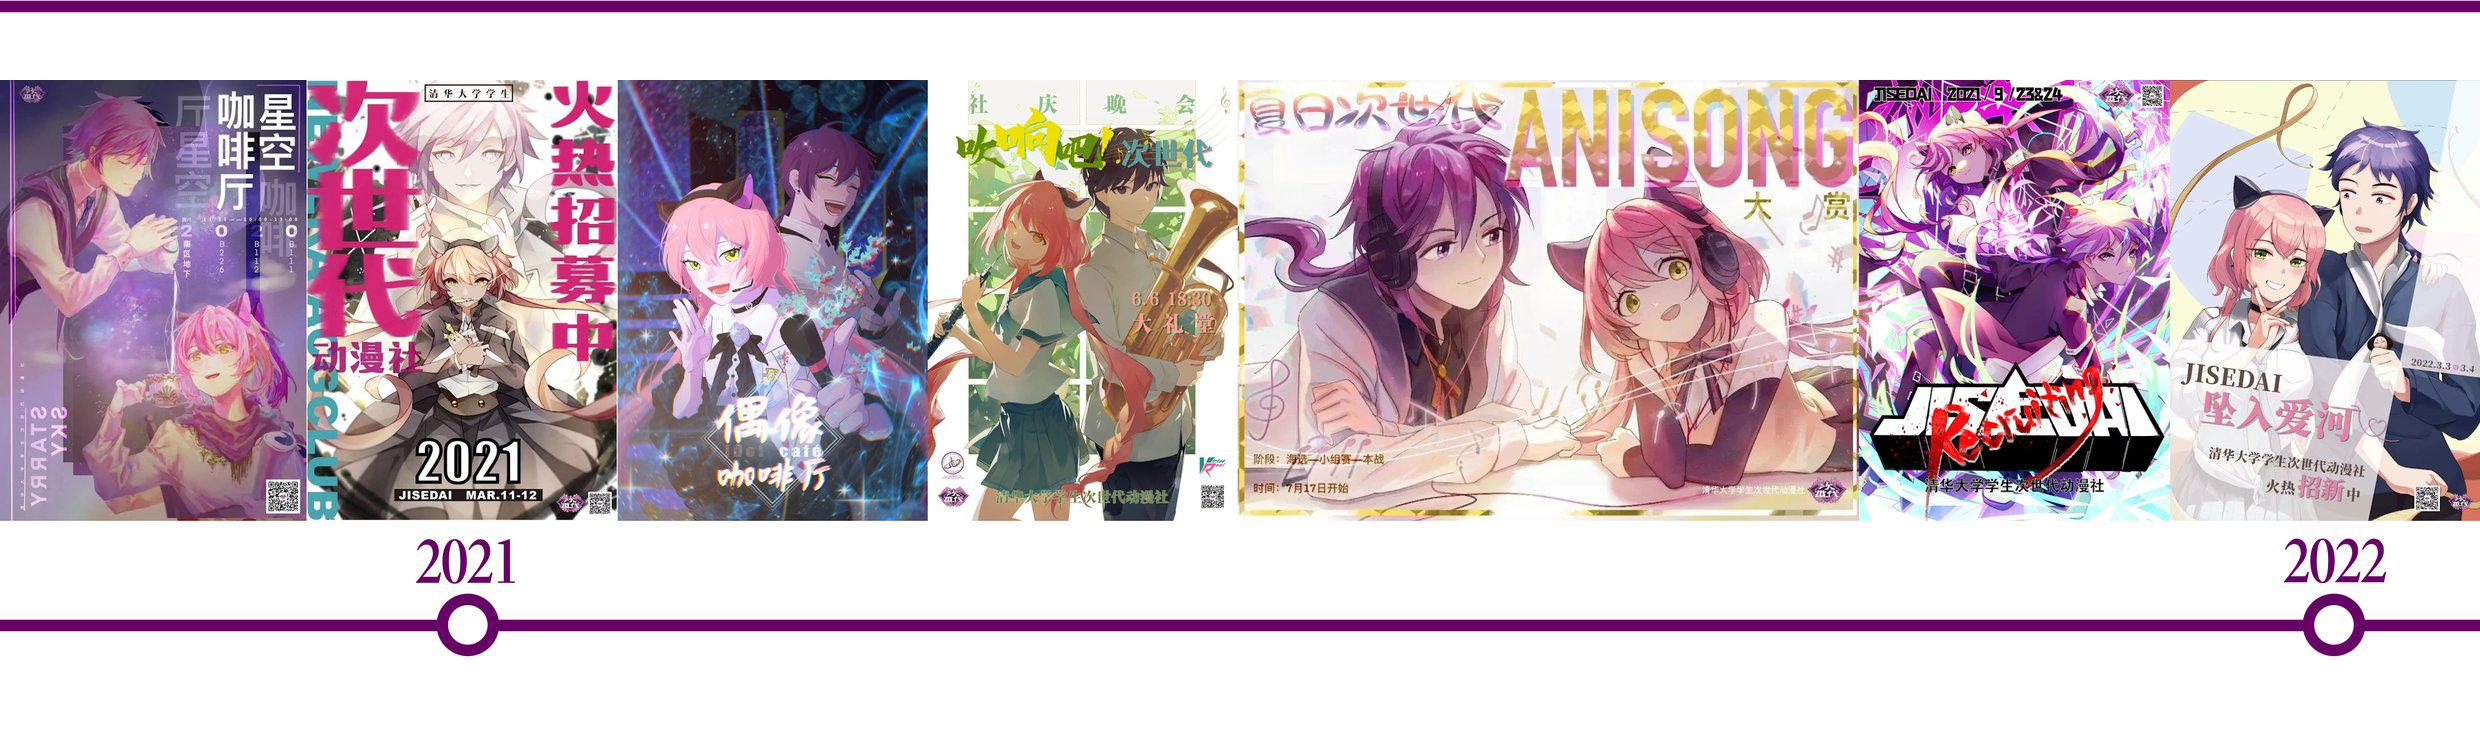
\includegraphics[width=\paperwidth]{tl4.jpg}
\end{textblock*}



\newpage
\fontsize{23pt}{24pt}\selectfont
\begin{center}
    \textbf{\textcolor{truepurple}{实验剧场乐队live}}\\
\end{center}
\vspace{-1em}
\adjustbox{valign=t}{
	\begin{minipage}[t]{0.45\textwidth}
		\vspace{0.5em}
		\raisebox{-\height}{
			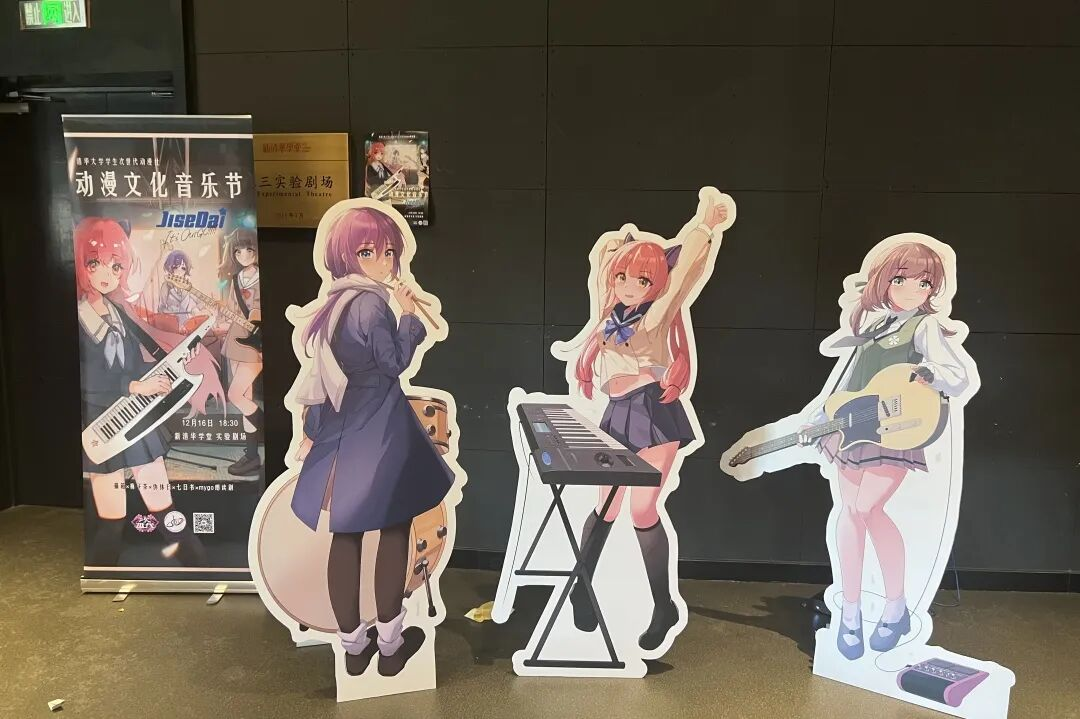
\includegraphics[width=\linewidth]{乐队4.jpg}}
    \par
		\vspace{0.5em}
		\raisebox{-\height}{
			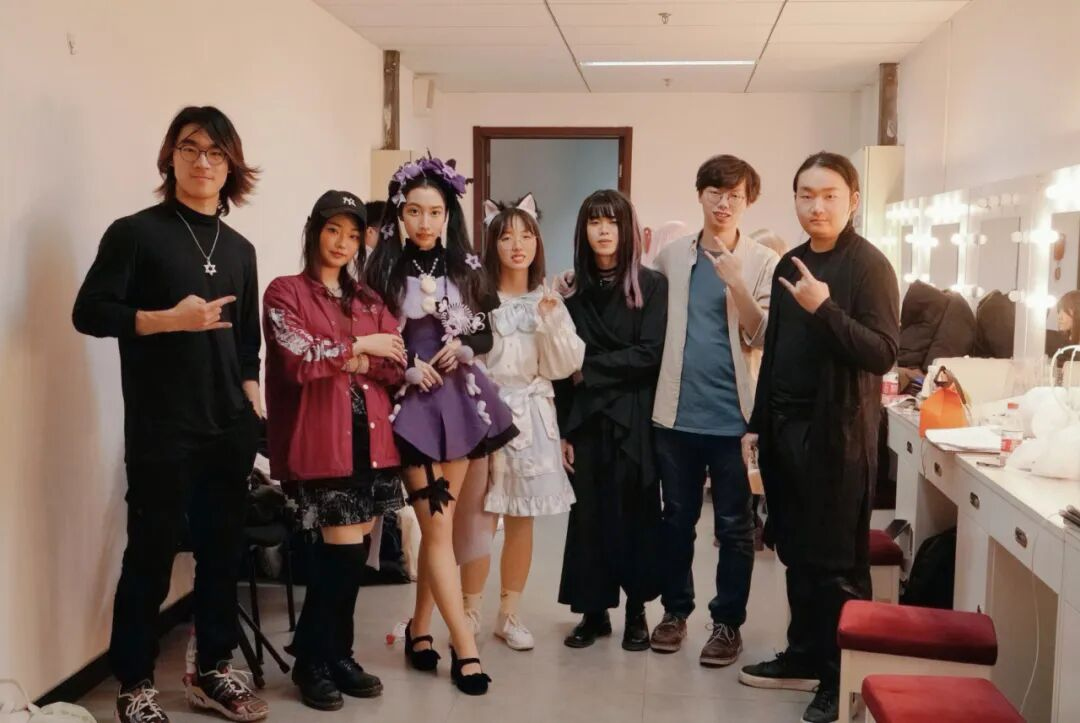
\includegraphics[width=\linewidth]{乐队5.jpg}}

		\normalsize
    \par
    \vspace{0.2em}
		\chind 作为乐队部的招牌项目,每学期一度、于新清华学堂实验剧场举行的乐队live都是一场乐队演出的狂欢。在这里,请你见证量大管饱的乐队表演:人声与演奏,拍动与旋律,演绎与原创……从ACGN到独立摇滚,从jpop到国漫经典,我们的歌单也构成着自我表达的电波。\\
    \chind 一首首曲子的呈现是各队队员一次次练习的结晶。希望我们的努力,足以回应大家为我们付出的每一张门票、每一秒时光、每一声应援。如果愿意的话,我们也欢迎台下的每一个你成为站到台上的一员。\\

	\end{minipage}}
\hfill
\adjustbox{valign=t}{
	\begin{minipage}[t]{0.45\textwidth}
    \vspace{0.4em}
		\raisebox{-\height}{
			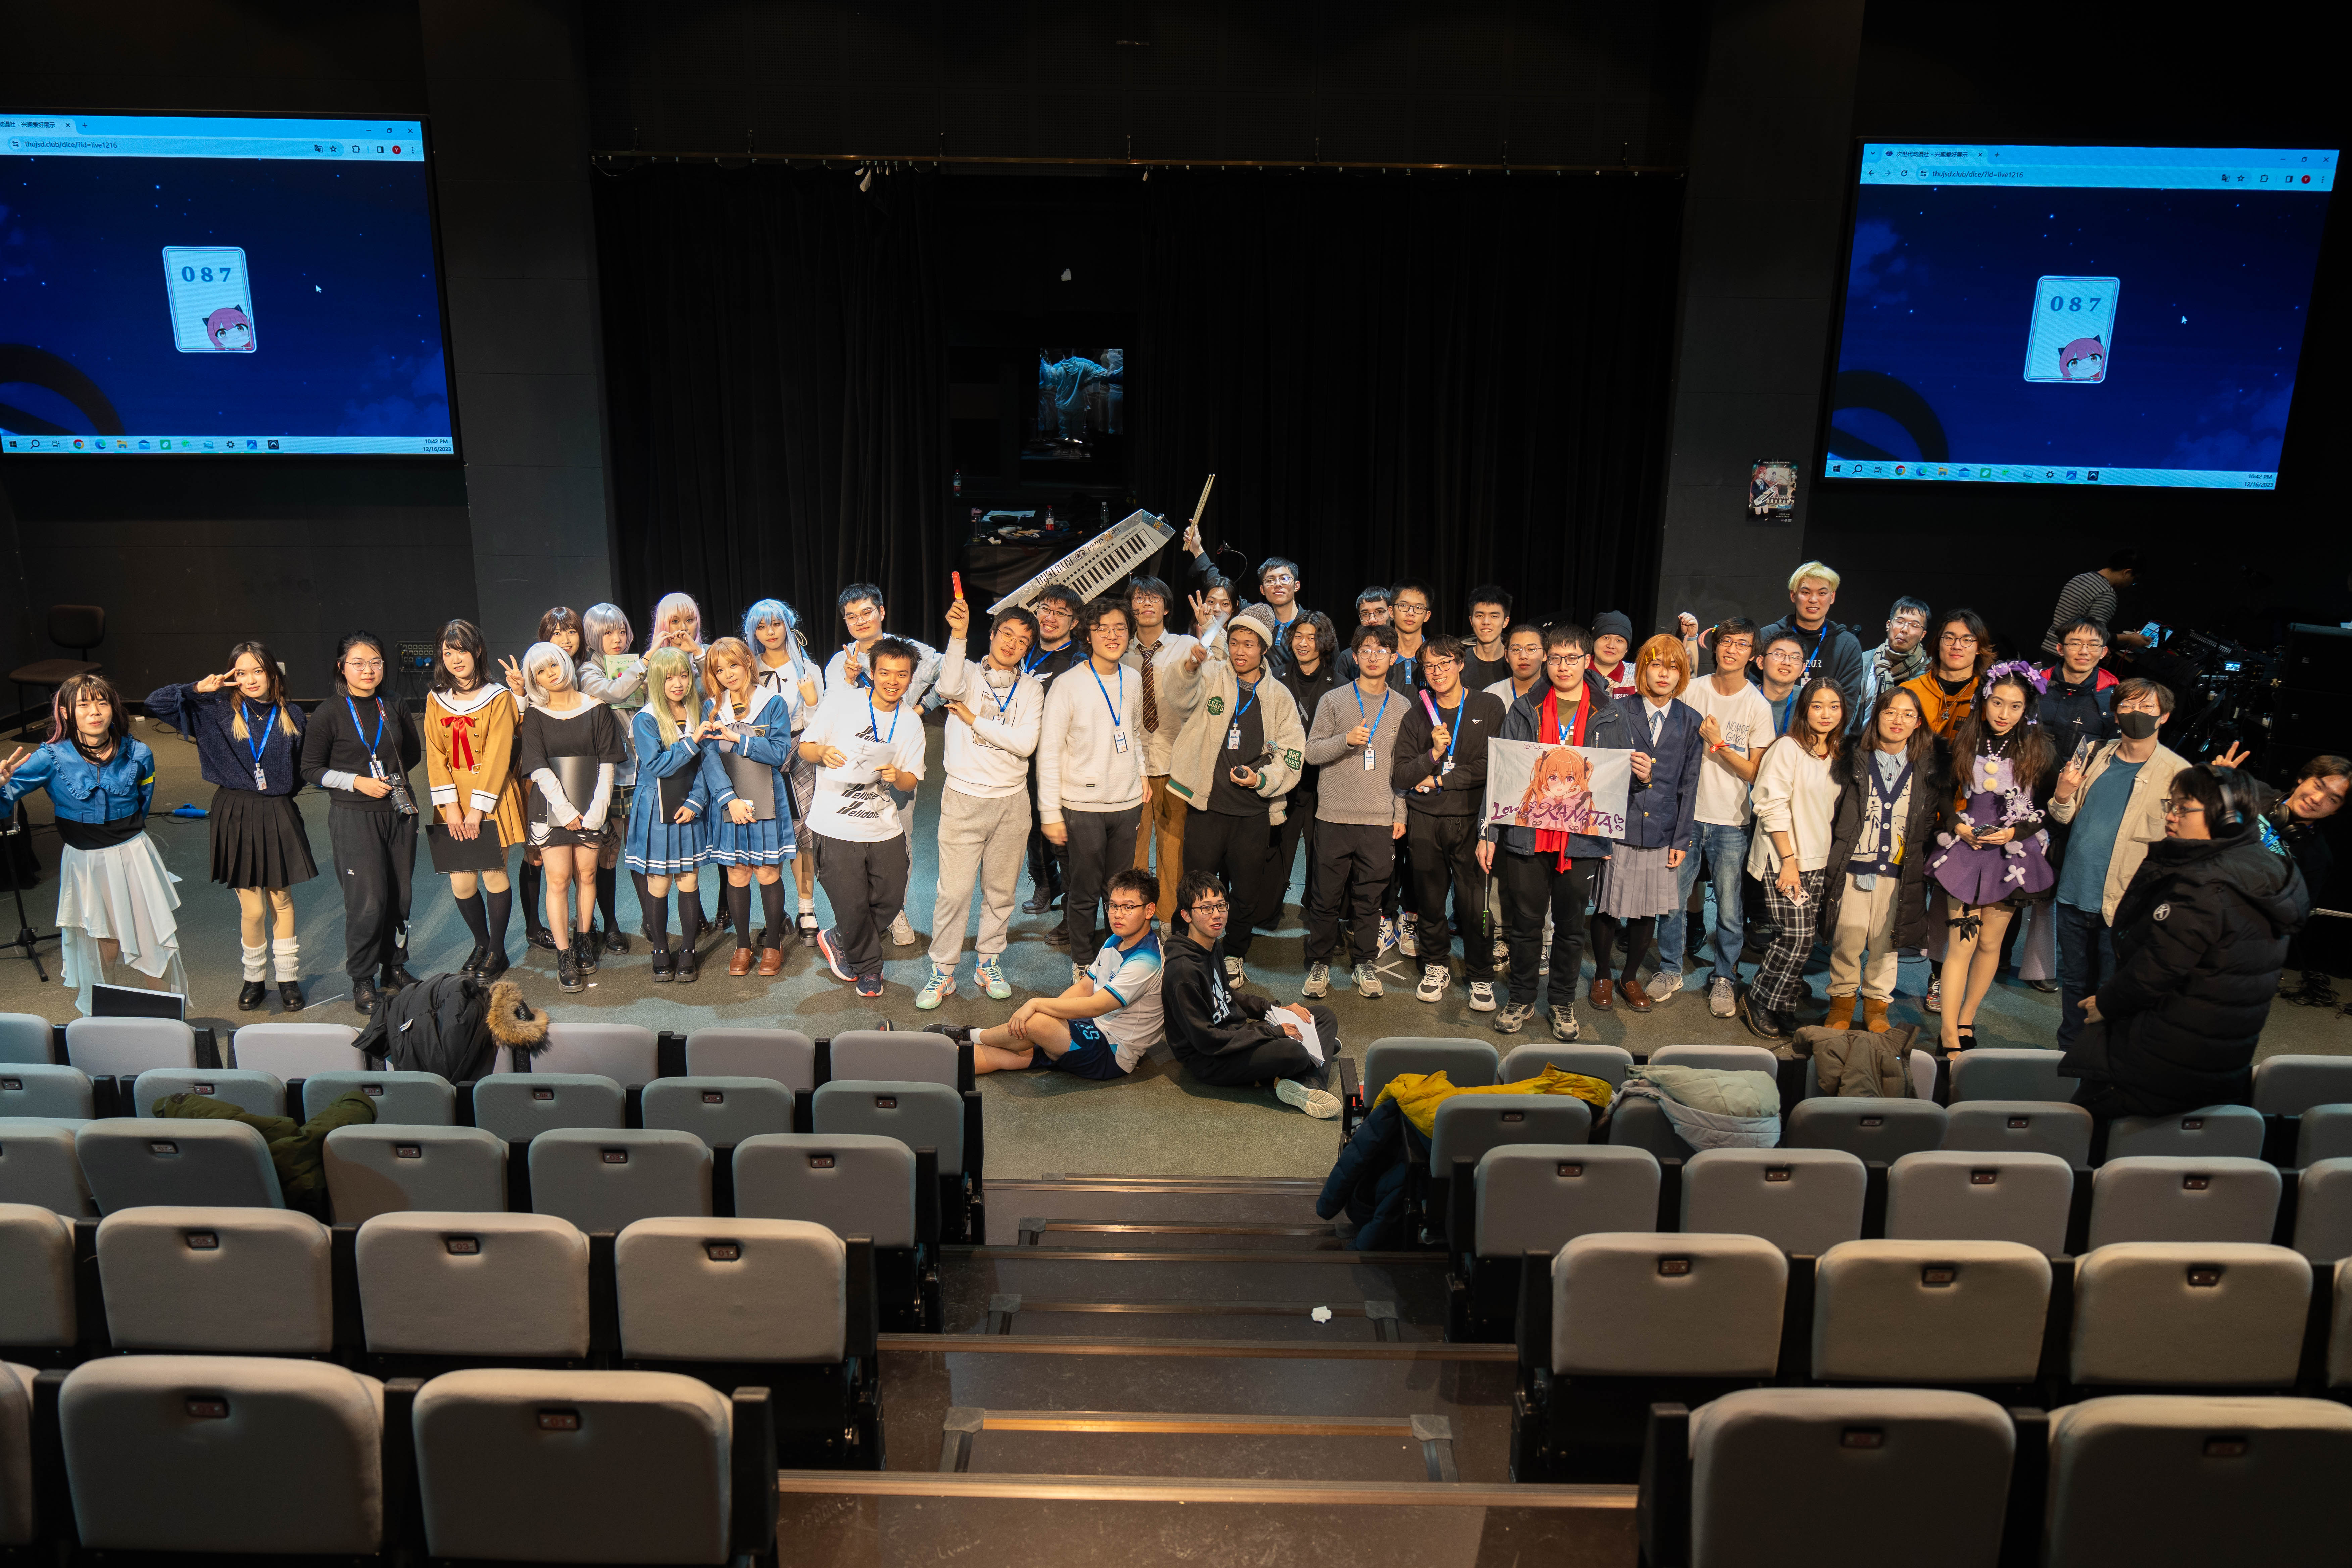
\includegraphics[width=\linewidth]{乐队1.jpg}}
		\par
		\vspace{0.5em}
		\raisebox{-\height}{
			\includegraphics[width=\linewidth]{乐队3.jpg}}
		\par
		\vspace{0.5em}
		\raisebox{-\height}{
			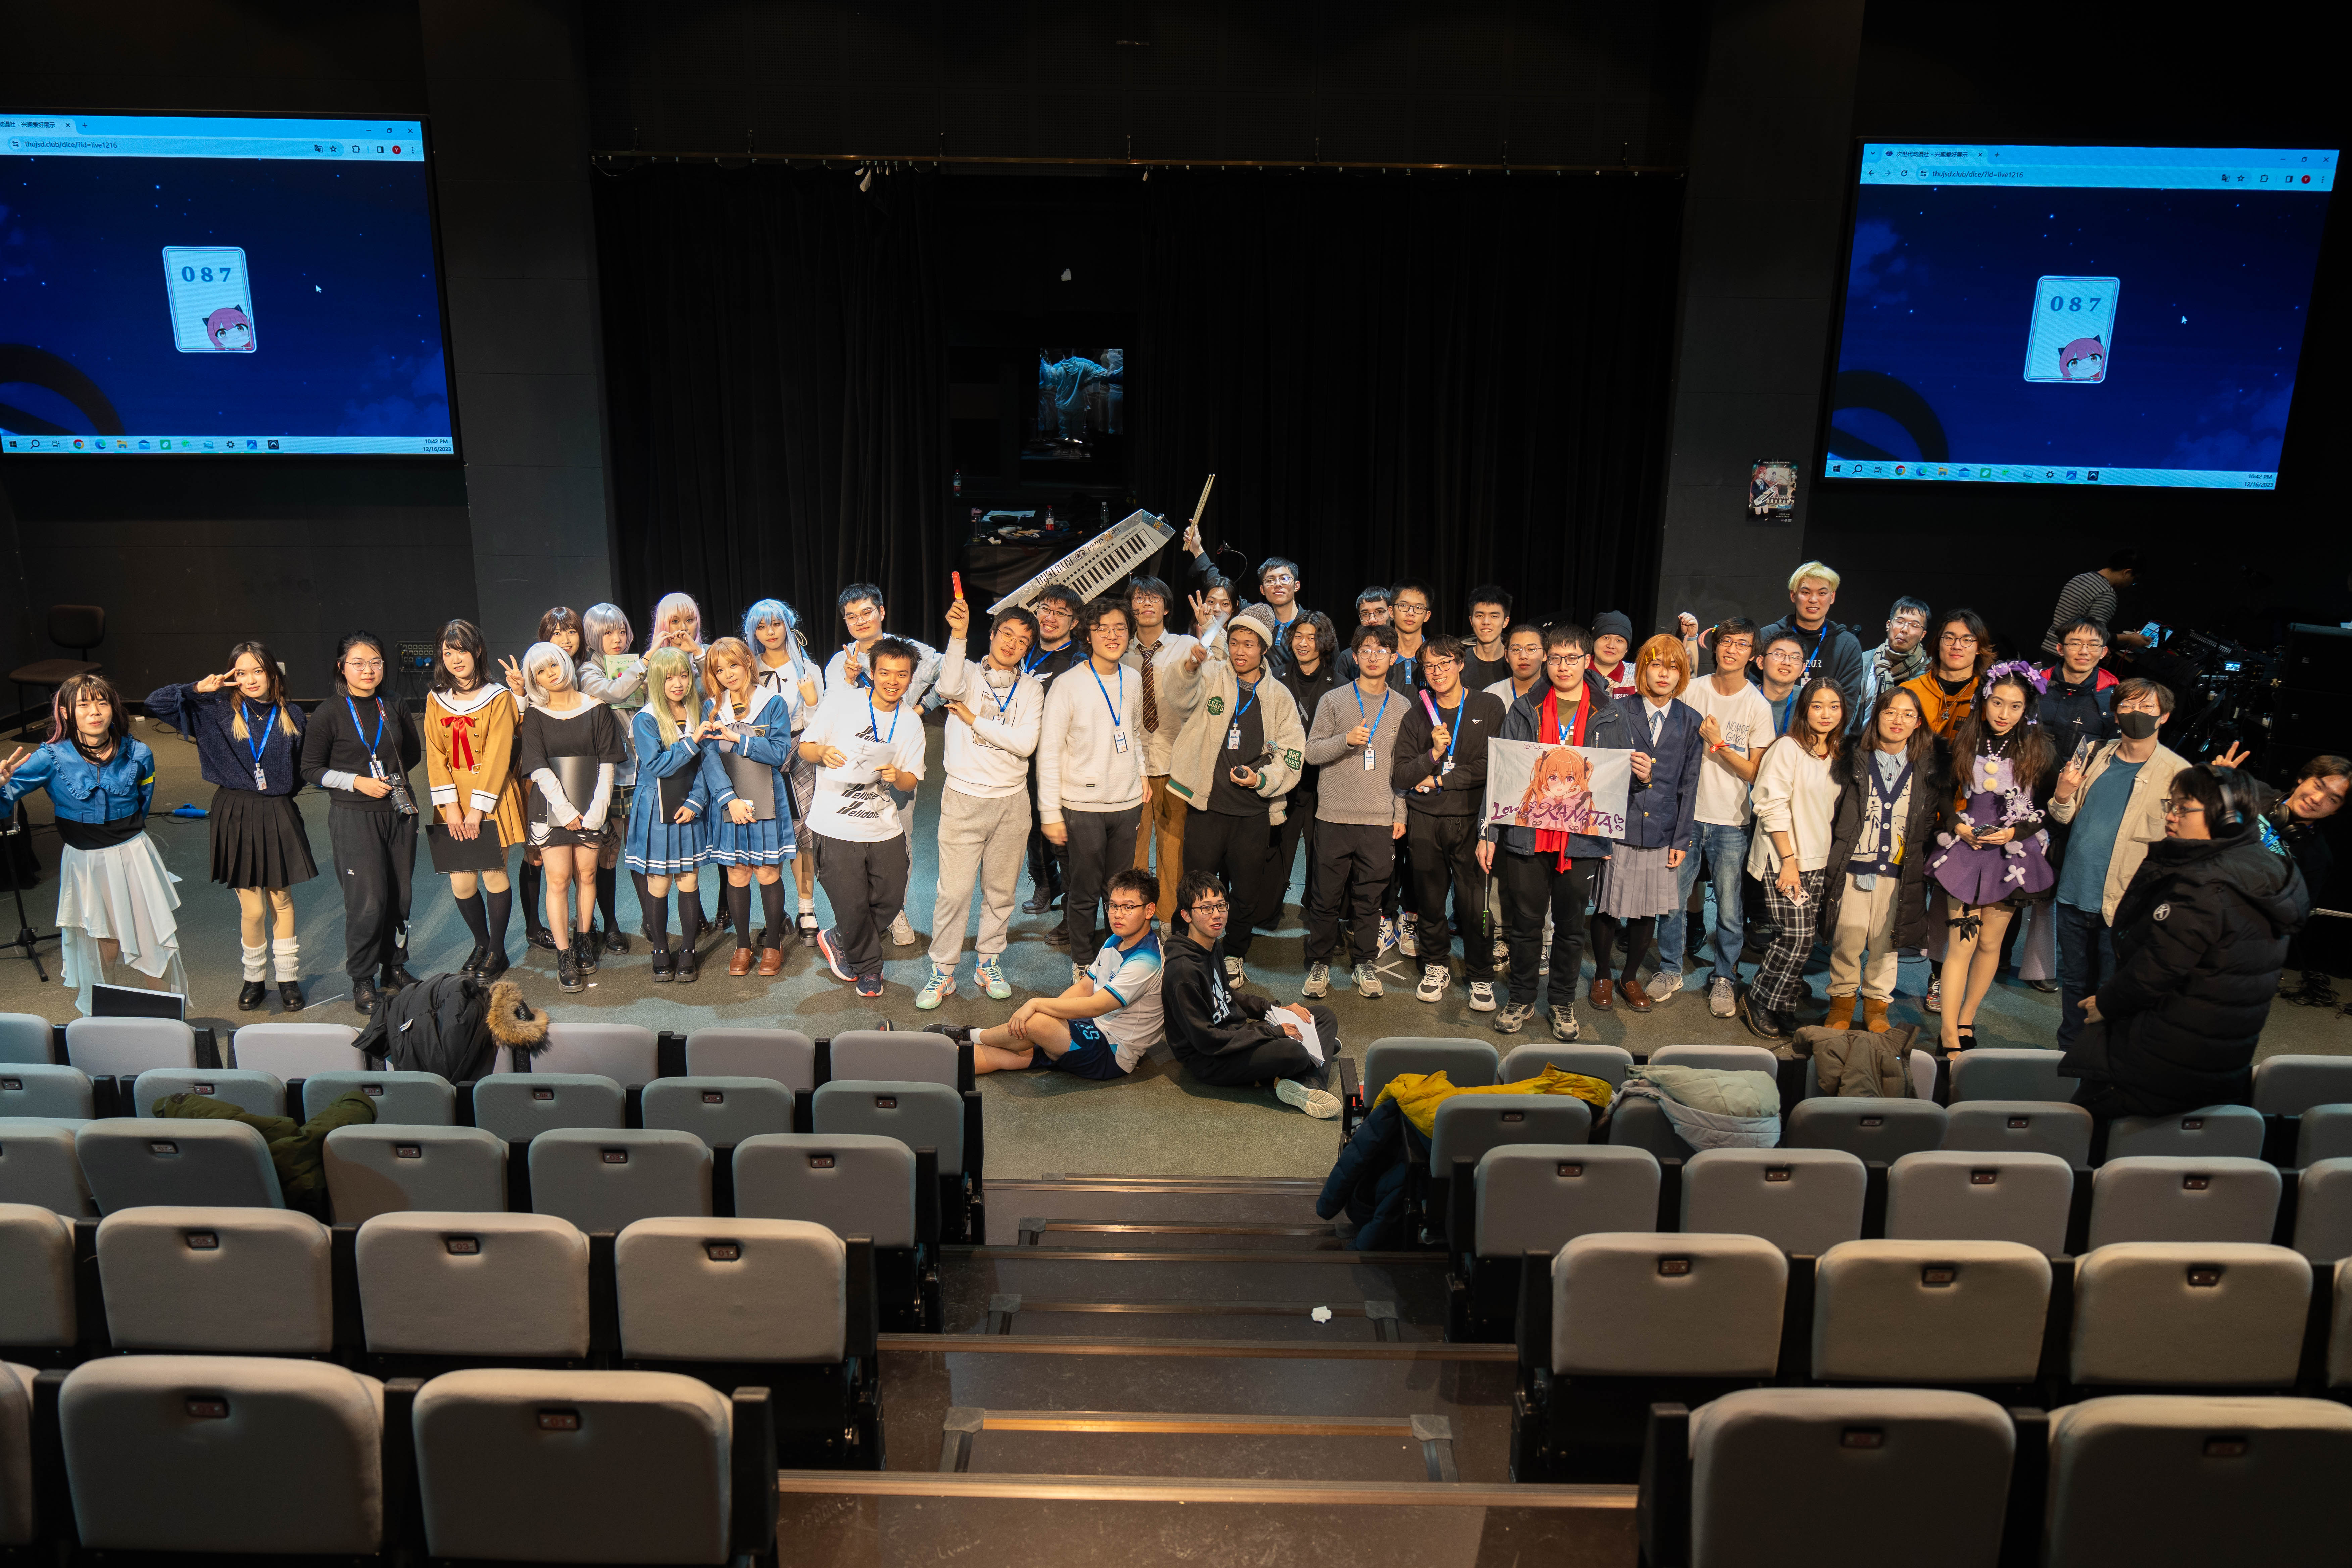
\includegraphics[width=\linewidth]{乐队2.jpg}}

	\end{minipage}%
}
\begin{textblock*}{\paperwidth}(0mm, \dimexpr\paperheight-78.5mm\relax) % 距顶部 = 纸高 - 30mm
  \noindent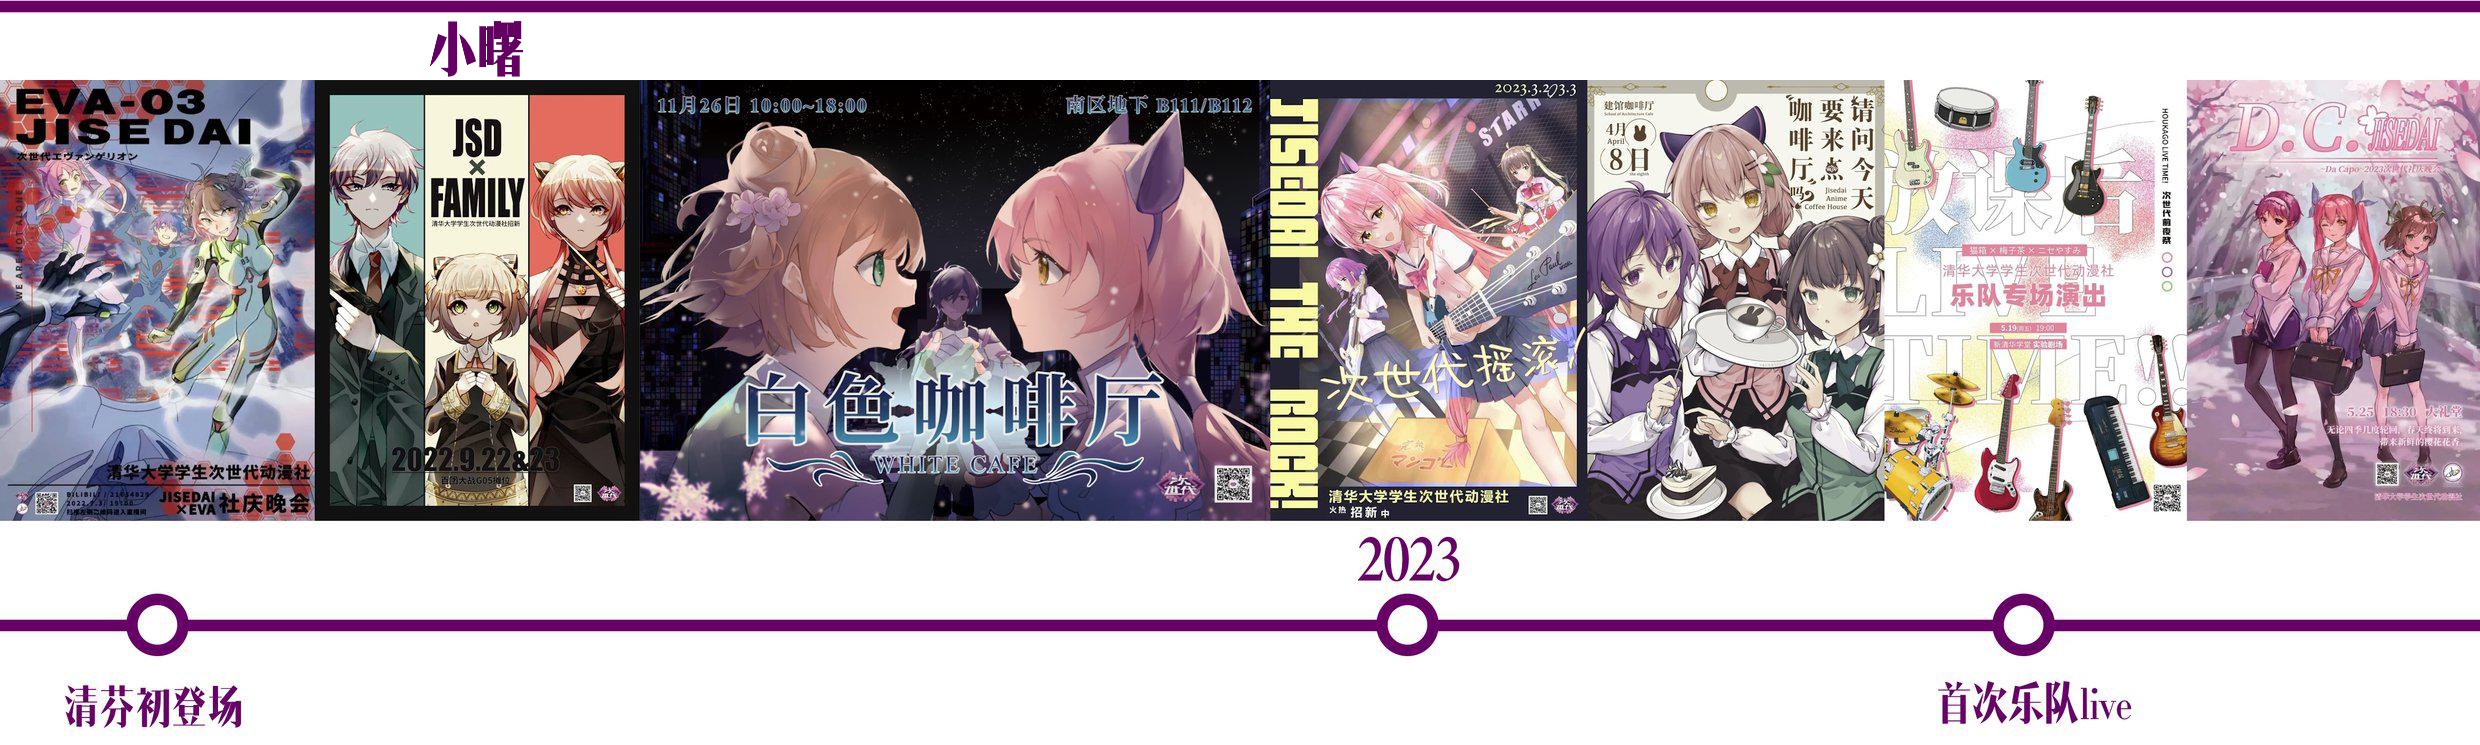
\includegraphics[width=\paperwidth]{tl5.jpg}
\end{textblock*}



\newpage
\fontsize{23pt}{24pt}\selectfont
\begin{center}
    \textbf{\textcolor{truepurple}{Idolive系列宅舞专场}}\\
\end{center}
\vspace{-0.5em}
\adjustbox{valign=t}{
	\begin{minipage}[t]{0.45\textwidth}
		\vspace{0.5em}
		\raisebox{-\height}{
			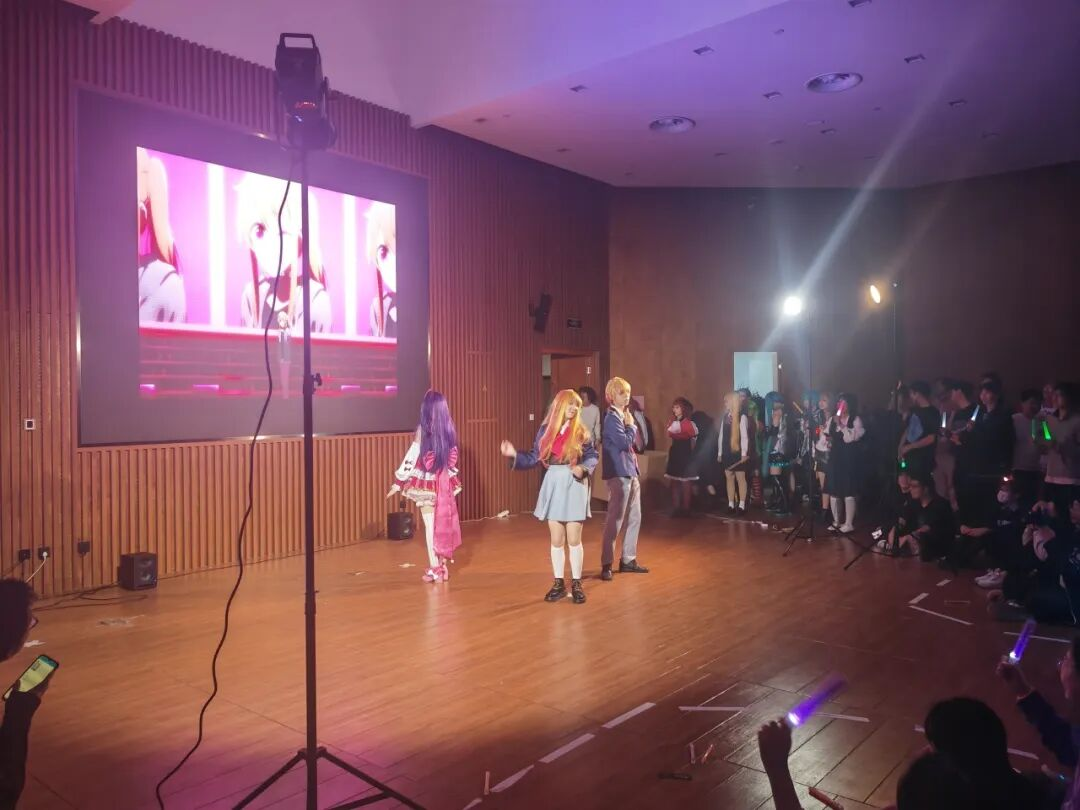
\includegraphics[width=\linewidth]{宅舞1.jpg}}
    \par
		\vspace{0.5em}
		\raisebox{-\height}{
			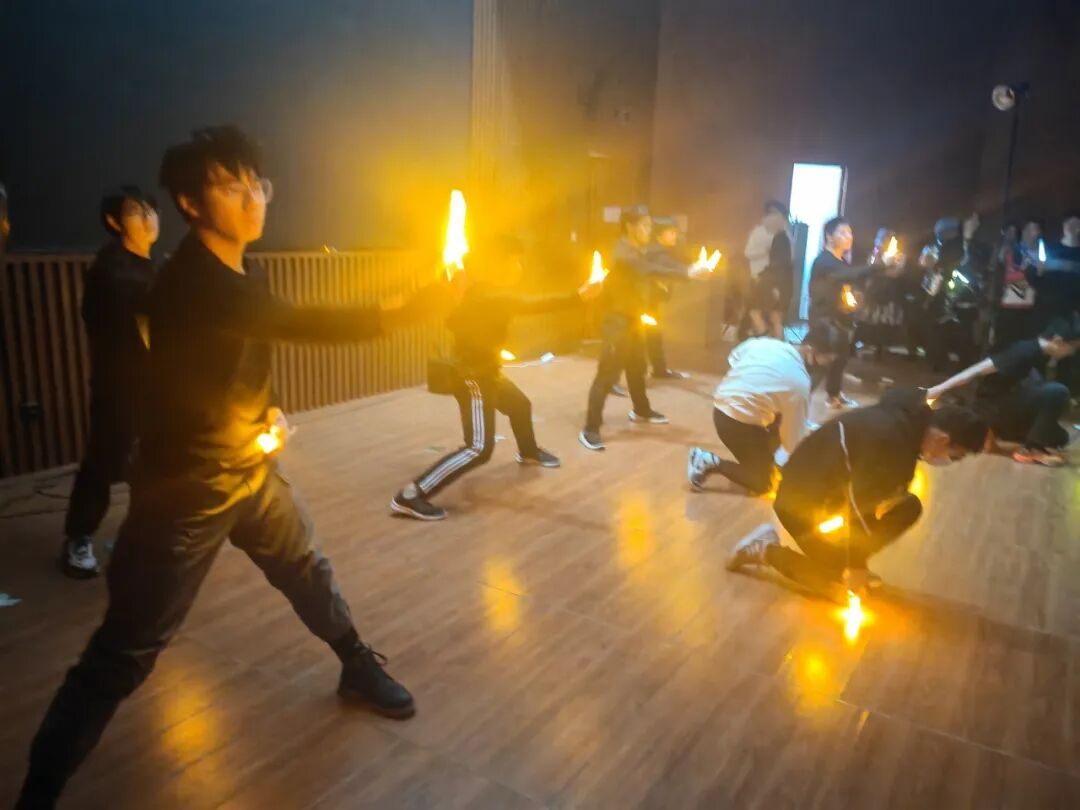
\includegraphics[width=\linewidth]{宅舞7.jpg}}
		\par
		\vspace{0.5em}
		\raisebox{-\height}{
			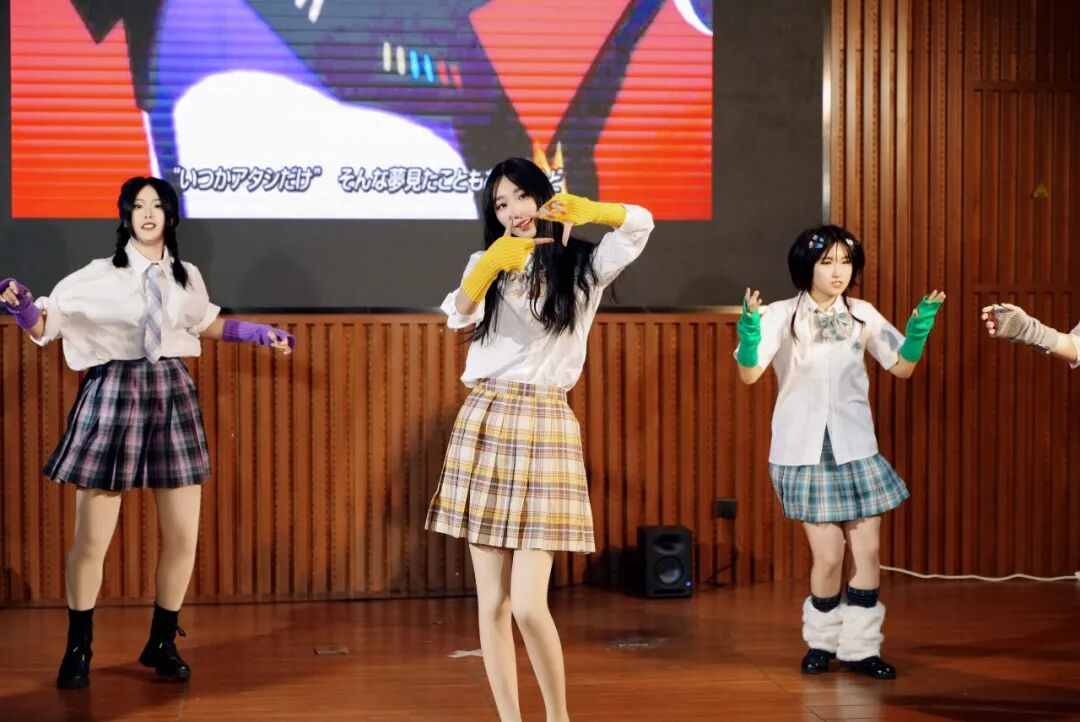
\includegraphics[width=\linewidth]{宅舞6.jpg}}

	\end{minipage}}
\hfill
\vspace{-0.5em}
\adjustbox{valign=t}{
	\begin{minipage}[t]{0.45\textwidth}
		\normalsize
    \par
		\chind Idolive系列是由次世代动漫社宅舞部自主研发的一款宅舞专场活动。专场发生在一个被称作B226的南区地下活动室,在这里,你将扮演超级元气小偶像,在自由的舞蹈中邂逅性格各异、能力独特的朋友们,逐步发掘宅舞的真相。清芬和桃子都曾经当过c位!\\
    \chind 宅舞专场分多段进行,中间设置了随机宅舞环节,随机串烧播放征集的配乐,可以自由登台下台,主打一个「想跳你就来」!\\
    \chind 此外, WOTA 艺部也会献上热血沸腾的光棒节目和应援。\\
		\par
    \vspace{-2em}
		\raisebox{-\height}{
			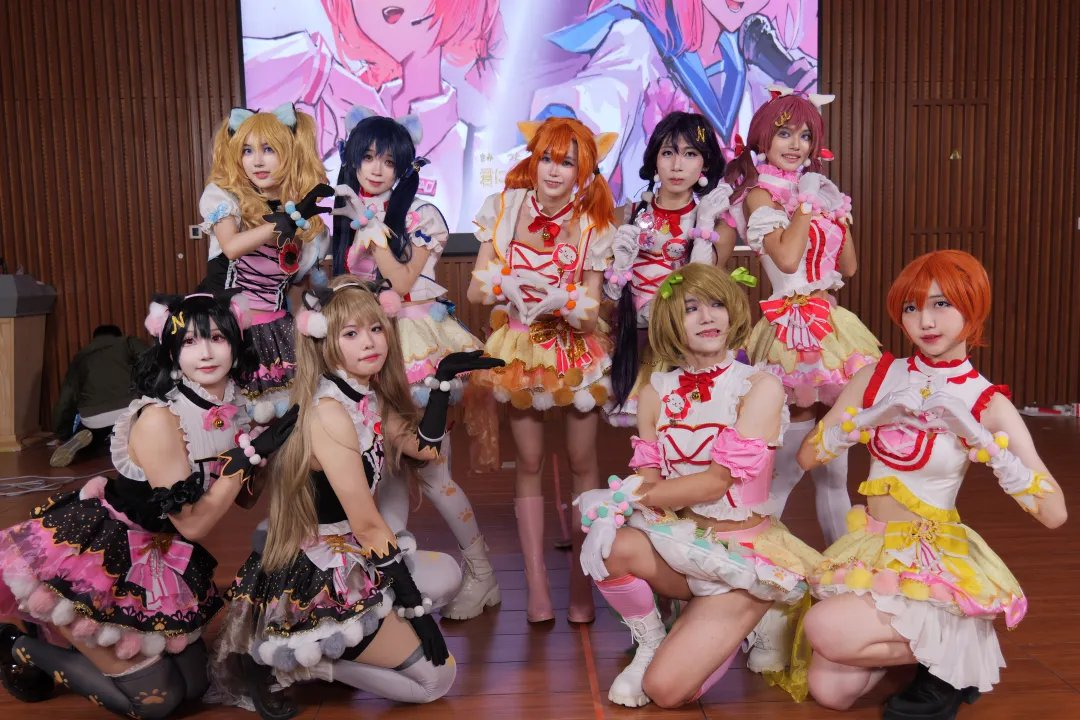
\includegraphics[width=\linewidth]{宅舞2.jpg}}

		\par
		\vspace{0.5em}
		\raisebox{-\height}{
			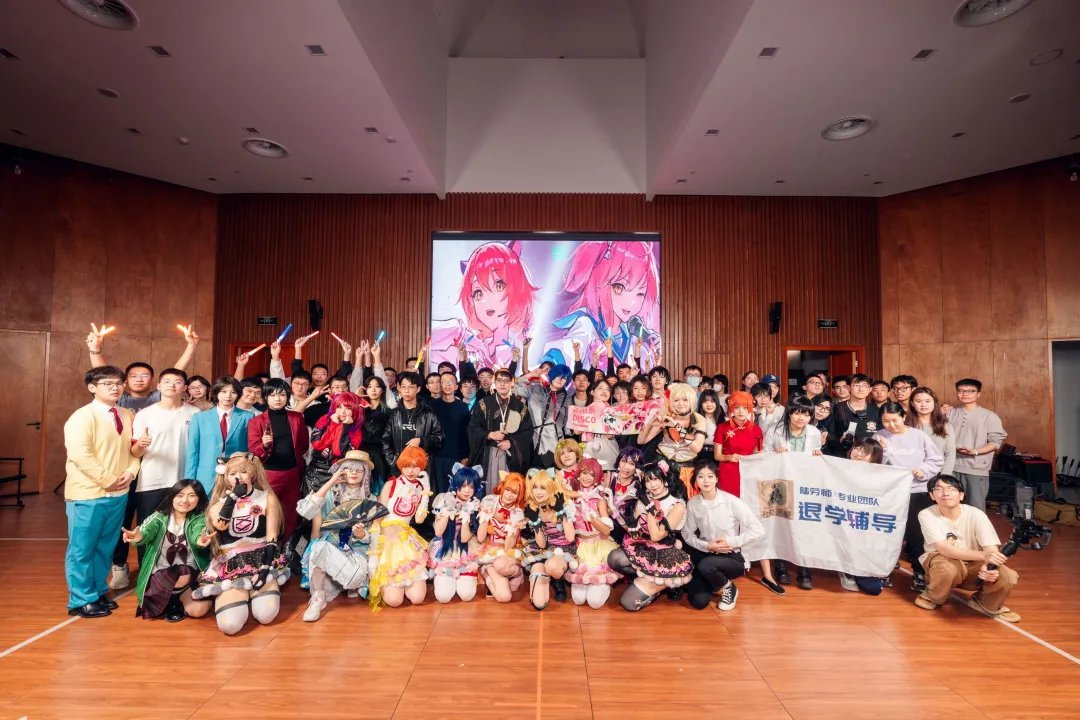
\includegraphics[width=\linewidth]{宅舞4.jpg}}

	\end{minipage}%
}
\begin{textblock*}{\paperwidth}(0mm, \dimexpr\paperheight-78.5mm\relax) % 距顶部 = 纸高 - 30mm
  \noindent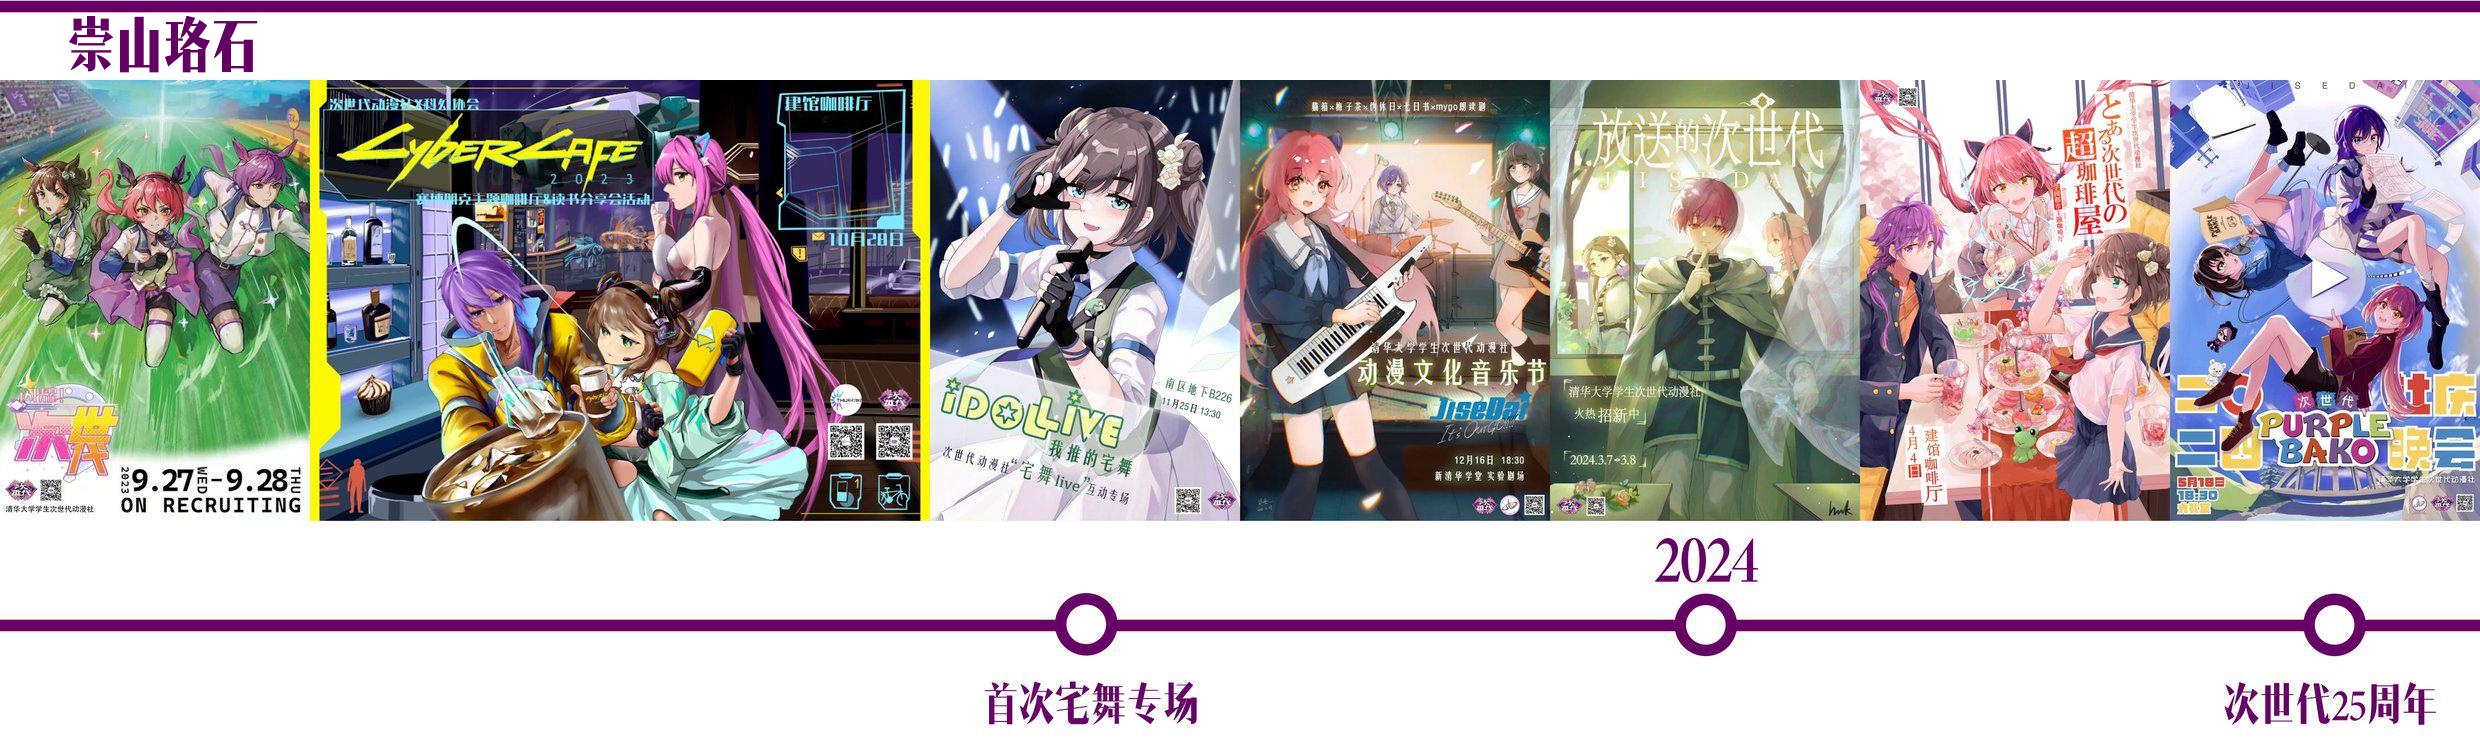
\includegraphics[width=\paperwidth]{tl6.jpg}
\end{textblock*}
\newpage
\par
\vspace{2em}

\adjustbox{valign=t}{
	\begin{minipage}[t]{0.4\textwidth}
		\vspace{-0.2em}
		\raisebox{-\height}{
			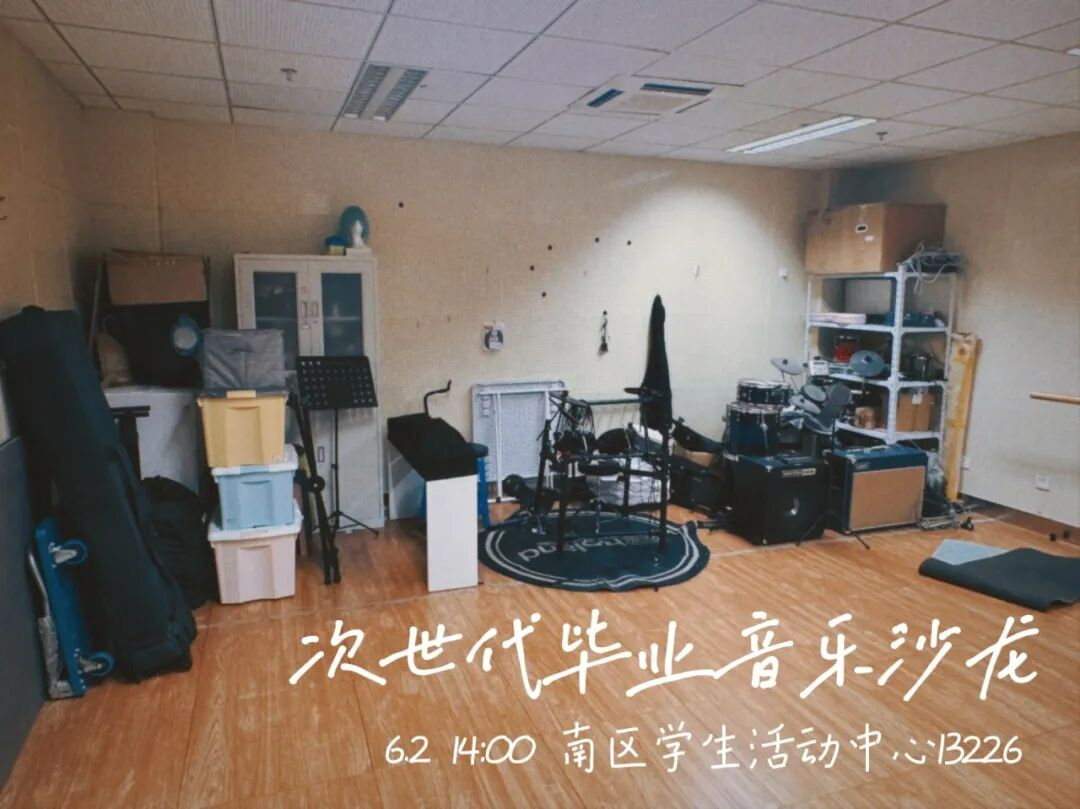
\includegraphics[width=1.1\linewidth]{沙龙.jpg}}
      \par
		\vspace{0.6em}
		\raisebox{-\height}{
			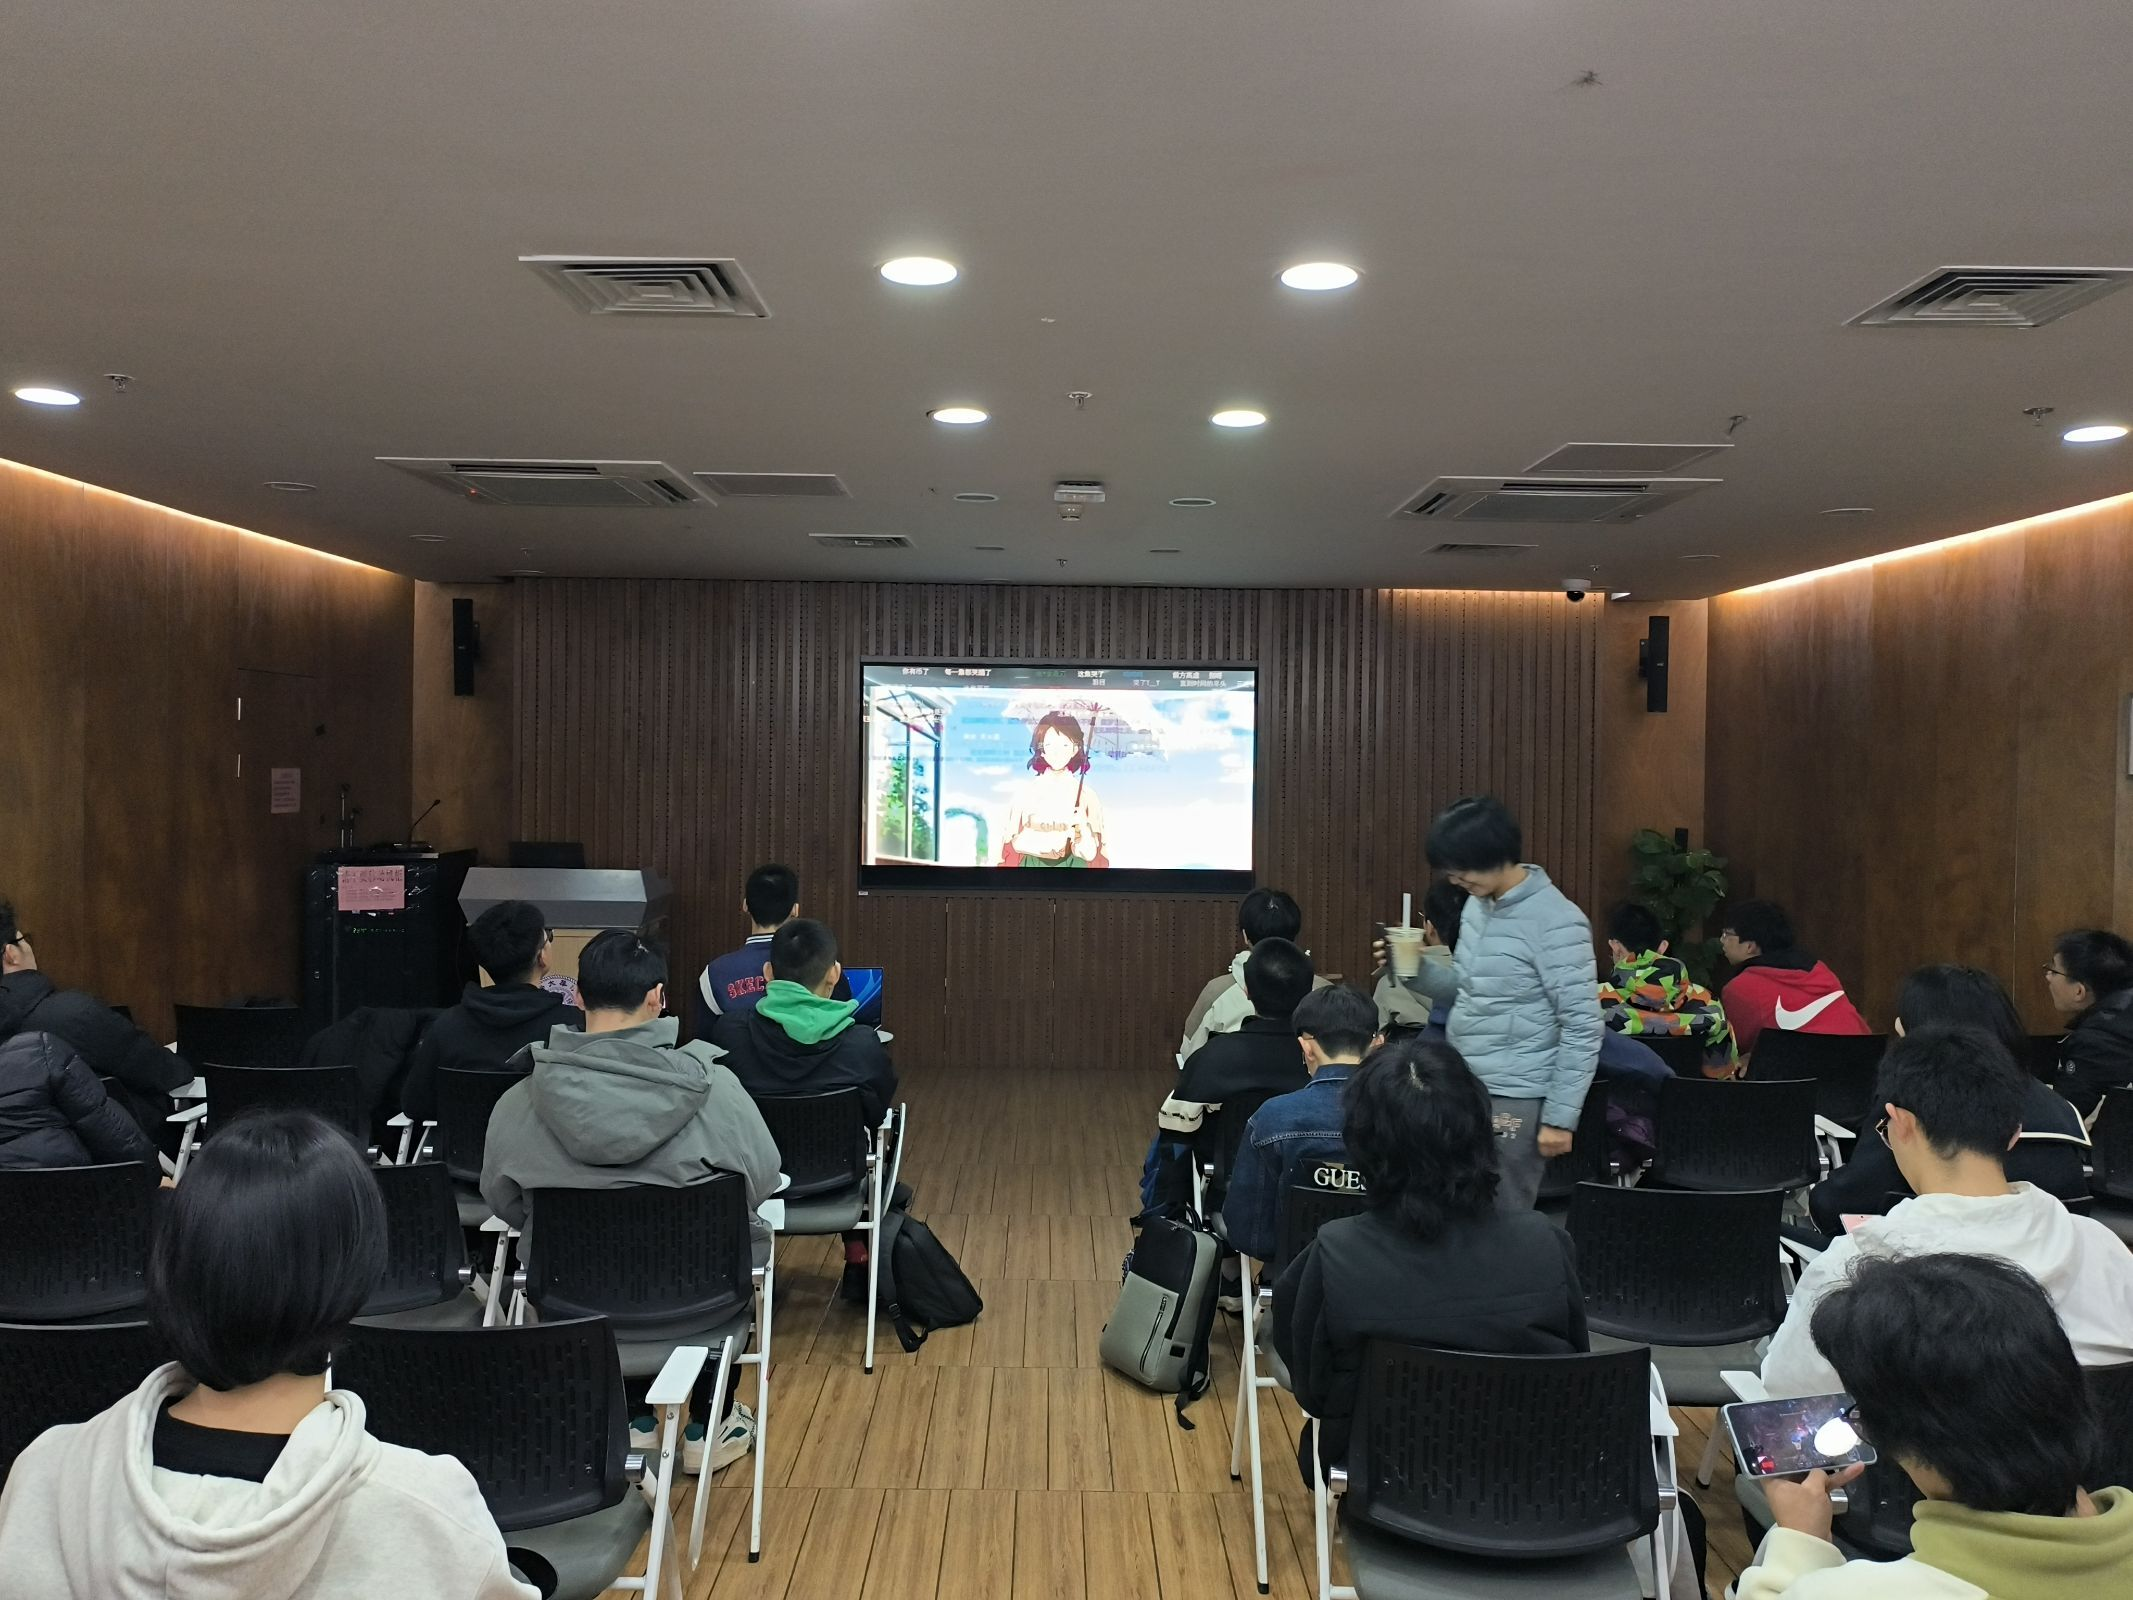
\includegraphics[width=1.1\linewidth]{放映会.jpg}}
      \par
		\vspace{0.6em}
		\raisebox{-\height}{
			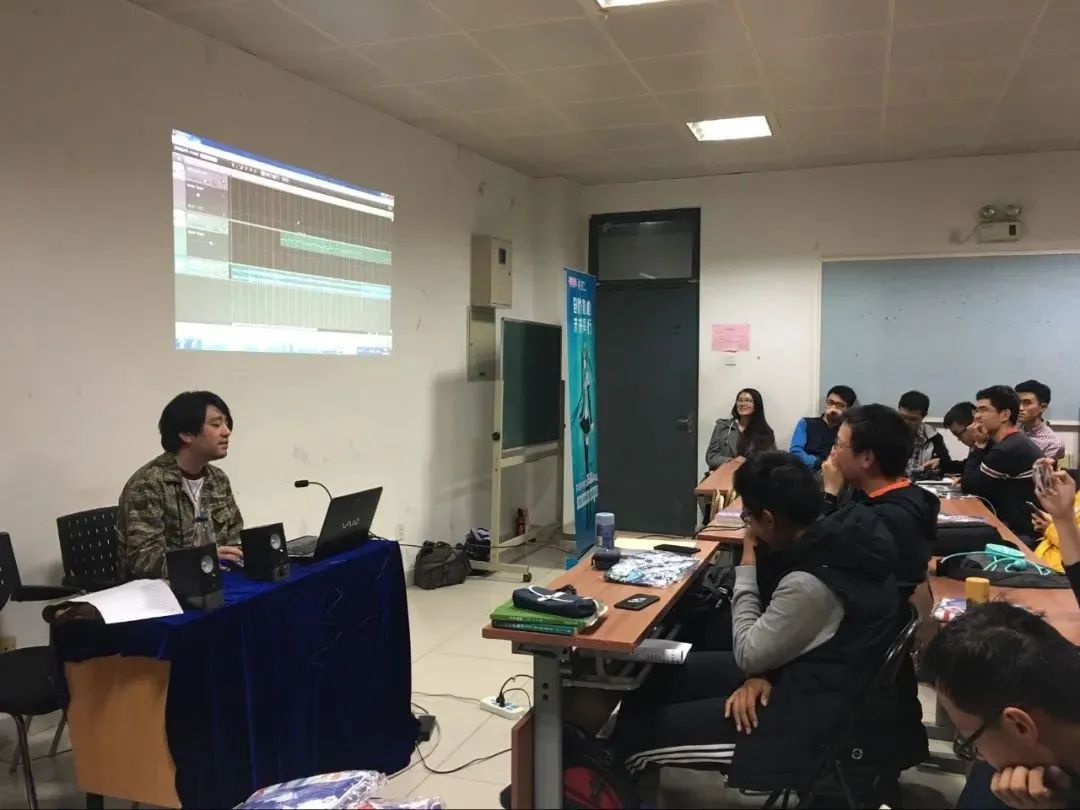
\includegraphics[width=1.1\linewidth]{讲座.jpg}}
	\end{minipage}%
}
\hfill
\adjustbox{valign=t}{
	\begin{minipage}[t]{0.5\textwidth}
    \fontsize{23pt}{24pt}\selectfont
    \begin{center}
\textbf{\textcolor{truepurple}{B226乐队部沙龙}}\\
    \end{center}
\par
		\vspace{-0.5em}
		\normalsize
		\chind 首次乐队部沙龙于上学期期末举办,主题为毕业季纪念,后续乐队部计划将该活动转化为常规活动。\\
    \chind 乐队部沙龙将以更轻松的氛围接纳更多的音乐元素,届时部内的临时企划和新手乐队将与大家见面,还会有anikura、现场点唱等活动等你到来。\\
   \par
    \fontsize{23pt}{24pt}\selectfont
    \vspace{-0.5em}
    \begin{center}
\textbf{\textcolor{truepurple}{周常放映会}}\\
    \end{center}
\par
		\vspace{-0.5em}
		\normalsize
		\chind 我们会在学期内每周开展经典动画电影,新剧场版动画或演唱会的放映活动,并建立了次世代放映组,为大家带来更好的观影体验。\\
    \chind 许多部门也会合作开展自己的放映。如果想要向同学安利你的品味\sout{公屏私用},欢迎加入放映组!\\
    \par
    \fontsize{23pt}{24pt}\selectfont
    \begin{center}
\textbf{\textcolor{truepurple}{例会/放映会/讲座}}\\
    \end{center}
\par
		\vspace{-0.5em}
		\normalsize
		\chind 例会是次世代\sout{除水群之外}的主要日常活动,其中分部例会更是重要的组成部分。虽然大家的兴趣各不相同,但总有一款能让你与同好们交流,结识更多同道中人。\\
    \chind 我们也经常邀请业界大佬来举办零距离讲座。先前邀请了知名Vocaloid~~P主匹诺曹P和知名插画师丁丁框老师,都获得了热烈反响,日后也敬请期待!\\
	\end{minipage}
}
\begin{textblock*}{\paperwidth}(0mm, \dimexpr\paperheight-78.5mm\relax) % 距顶部 = 纸高 - 30mm
  \noindent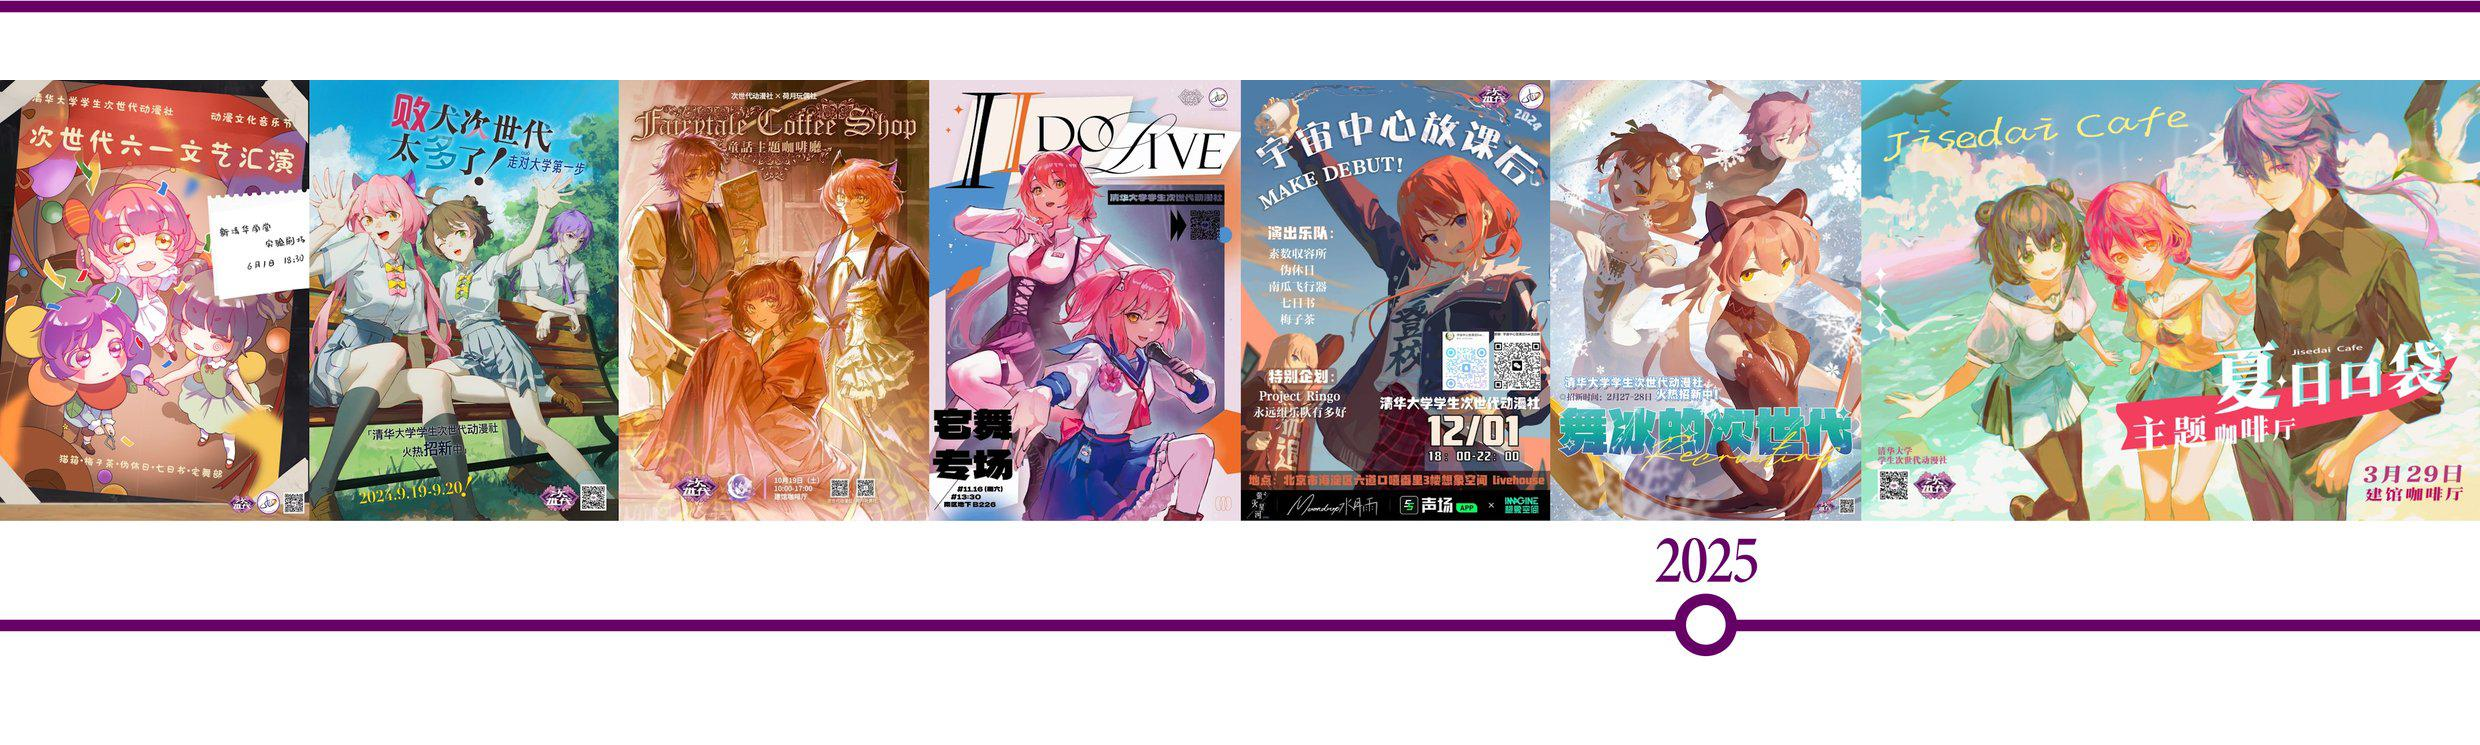
\includegraphics[width=\paperwidth]{tl7.jpg}
\end{textblock*}
\newpage
    \fontsize{23pt}{24pt}\selectfont
    \begin{center}
\textbf{\textcolor{truepurple}{往期活动}}\\
    \end{center}
    \par
\adjustbox{valign=t}{
	\begin{minipage}[t]{0.45\textwidth}
		
		\raisebox{-\height}{
			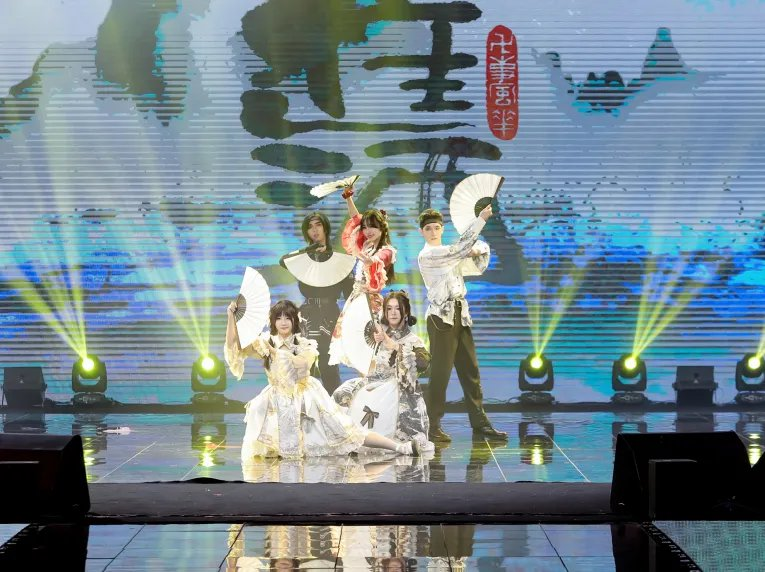
\includegraphics[width=\linewidth]{新年联欢晚会.jpg}}
		\vspace{-0.5em}
		\picbox{\small \ding{115} 出演新年联欢晚会}
  		\par
		\vspace{-0.5em}
		\raisebox{-\height}{
			
\includegraphics[width=\linewidth]{舞萌.jpg}}
		\vspace{-0.5em}
		\picbox{\small ~\ding{115} ~ 舞萌DX比赛~}
	\end{minipage}}
\hfill
\vspace{1em}
\adjustbox{valign=t}{
	\begin{minipage}[t]{0.45\textwidth}
		\par
    
		\raisebox{-\height}{
			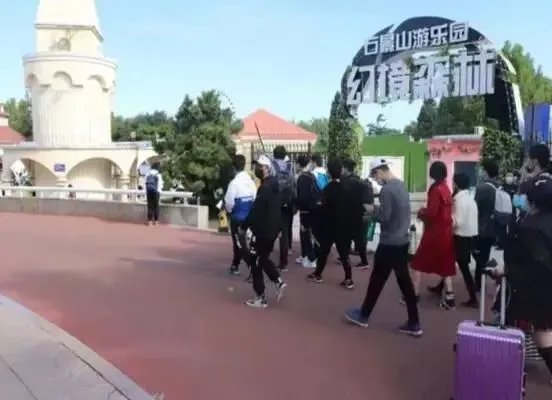
\includegraphics[width=\linewidth]{合宿.jpg}}
		\vspace{-0.5em}
		\picbox{\small ~\ding{115} ~ 合宿(会复刻的!)~}
		\normalsize
    \par
		\vspace{0em}
		\raisebox{-\height}{
			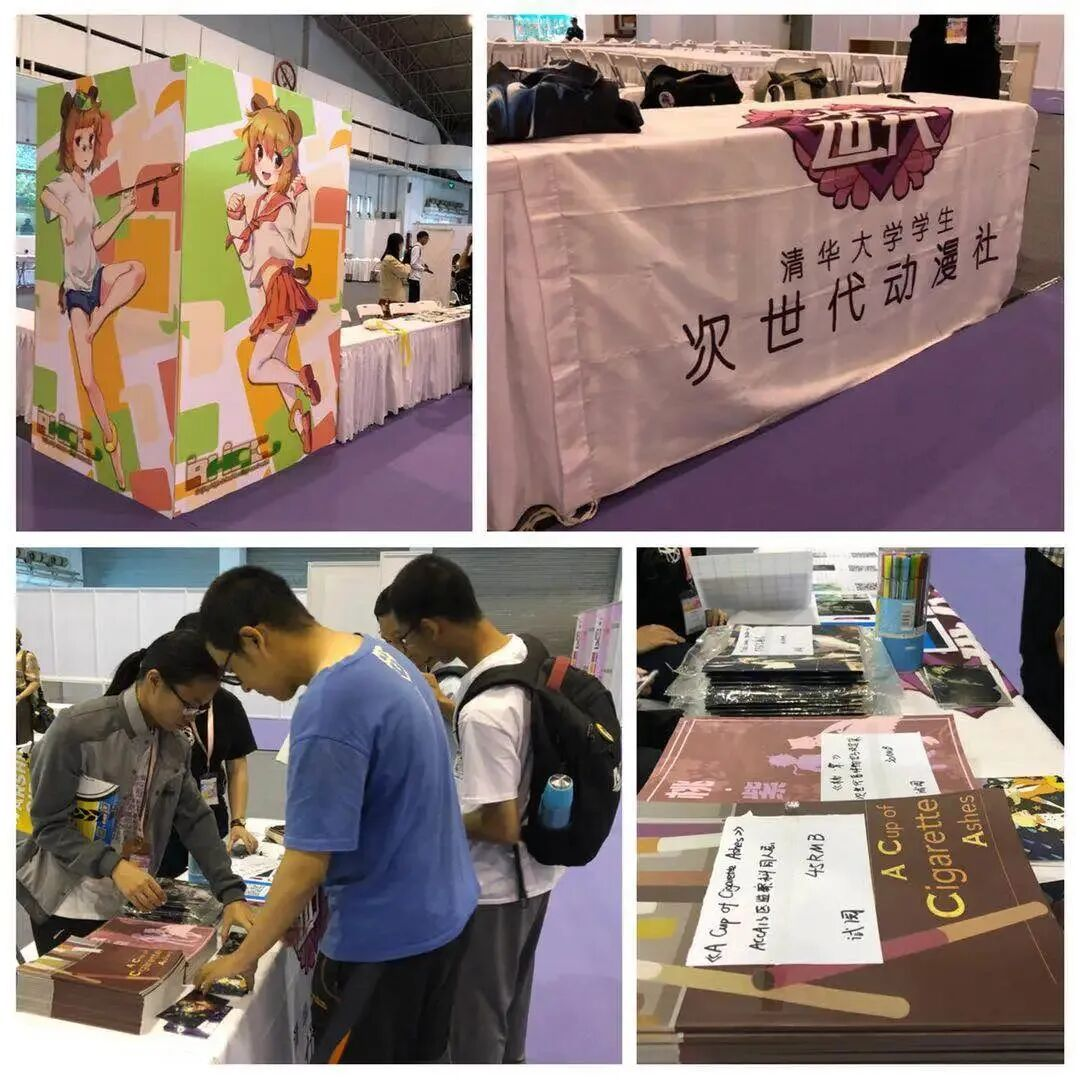
\includegraphics[width=0.8\linewidth]{BHCC.jpg}}
		\vspace{-0.5em}
		\picbox{\small ~\ding{115} ~ 参与BHCC北京高校联盟漫展~}

	\end{minipage}%
}
\normalsize
\chatbubble[right]{zijing.jpg}{紫荆}{
\textbf{甚至是,你想要举办的全新活动……?}
}{zi}
\begin{textblock*}{\paperwidth}(0mm, \dimexpr\paperheight-78.5mm\relax) % 距顶部 = 纸高 - 30mm
  \noindent
\includegraphics[width=\paperwidth]{tl8.jpg}
\end{textblock*}